% Dokumentklassen:
% article, report, beamer, book, letter etc.
% https://en.wikibooks.org/wiki/LaTeX/Document_Structure
\documentclass[a4paper]{article}

% Seitenränder Abstand setzen
\usepackage[margin=80pt]{geometry}

% Deutsches Sprachpaket
\usepackage[ngerman]{babel}
% UTF8 Input Encoding
\usepackage[utf8]{inputenc}

\usepackage{amssymb}
\usepackage{amsmath}

% Schriftbild ändern
% https://en.wikibooks.org/wiki/LaTeX/Fonts
\usepackage[scaled]{helvet}
% (Sans) Serifen oder anderes
% \rmdefault: Serifen
% \sfdefault: Sans-Serifen
% \ttdefault: Typewriter
\renewcommand{\familydefault}{\sfdefault}
% Fontencoding (für ä, ö, ü etc.)
\usepackage[T1]{fontenc}

% Gänsefüsschen richtig kompilieren
\usepackage [autostyle]{csquotes}
\MakeOuterQuote{"}

% Hyperlinks farblos
\usepackage[hidelinks]{hyperref}
\hypersetup{colorlinks=false}

% Package für Aufzählungen
\usepackage{enumitem}
% kein Abstand zwischen Aufzählungen
% Sollen doch Abstände vorhanden sein: nach Aufzählung {itemsep=1em}
\setlist{nosep}

% Grafik-Packages, für Figures, Subfigures und PDF als Import
\usepackage{graphicx}
\usepackage{subcaption}
\usepackage{pdfpages}
\usepackage{mwe}

% Package und Einstellungen für Java-Code-Darstellung
% Werden erstellt mit \begin{lstlisting}
\usepackage{listings}
\usepackage{color}
\definecolor{dkgreen}{rgb}{0,0.6,0}
\definecolor{gray}{rgb}{0.5,0.5,0.5}
\definecolor{mauve}{rgb}{0.58,0,0.82}
\lstset{frame=tb,
	language=Java,
	aboveskip=3mm,
	belowskip=3mm,
	showstringspaces=false,
	columns=flexible,
	basicstyle={\small\ttfamily},
	numbers=none,
	numberstyle=\tiny\color{gray},
	keywordstyle=\color{blue},
	commentstyle=\color{dkgreen},
	stringstyle=\color{mauve},
	breaklines=true,
	breakatwhitespace=true,
	tabsize=3
}

\title{\textbf{Zusammenfassung DL4G} \\
		Deep Learning for Games}
\date{\today}
\author{Maurin D. Thalmann}

\begin{document}
	
	\pagenumbering{gobble}
	\maketitle
	
	\newpage
	\pagenumbering{arabic}
	\tableofcontents
	
	\newpage
	
	\section{Sequential Games with perfect information}
	
		\subsection{Finite Sequential Games}
		
		\begin{itemize}
			\item Eine endliches Set an \textbf{Spielern}, jeder mit einem endlichen Set an möglichen \textbf{Aktionen}
			\item Spieler wählen ihre Aktionen \textbf{sequenziell} (einer nach dem anderen, in Zügen)
			\item Eine endliche Anzahl an \textbf{Zügen} wird gespielt
			\item Spätere Spieler \textbf{beobachten} die Züge der früheren Spieler (Perfect Recall)
			\item Eine \textbf{Strategie} sagt dem Spieler, welche Aktion er in seinem Zug spielen soll
			\item Ein \textbf{Strategieprofil} ist eine gewählte Strategie eines jeden Spielers
			\item Ein \textbf{Utility} oder \textbf{Payoff Function} bestimmt den Ausgang jedes Aktionprofils
		\end{itemize}
	
		\subsection{Complexity Factors in Game Analysis}
		
		\begin{enumerate}
			\item Anzahl Spieler
			\begin{itemize}
				\item Spiele mit 4 Spielern sind schwieriger zu analysieren als solche mit 2 Spielern
			\end{itemize}
			\item Grösse des Suchraums
			\begin{itemize}
				\item Bestimmt durch Anzahl gespielte Züge und Anzahl Aktionen für jeden Spieler
			\end{itemize}
			\item Kompetitive Spiele vs. Kooperative Spiele
			\begin{itemize}
				\item Kompetitive Spiele involvieren Spieler mit komplett gegensätzlichen Interessen 
			\end{itemize}
			\item Stochastische Spiele vs. Deterministische Spiele
			\begin{itemize}
				\item Stochastische Spiele beinhalten Zufälle, bspw. Verteilung der Karten, Würfel rollen
			\end{itemize}
			\item Perfekte vs. imperfekte Informationsspiele
			\begin{itemize}
				\item Imperfekte Information heisst das Spiel ist nur teilweise überwachbar, bspw. kennen wir nicht die Karten eines gegnerischen Spielers beim Poker oder Jass
			\end{itemize}
		\end{enumerate}
	
		\subsection{Illustration of State Space Complexity}
		
		\begin{table}[htb!]
			\begin{tabular}{ |c|c|}
				\textbf{Game} & \textbf{\begin{tabular}[c]{@{}c@{}}State Space\\ (as log to base 10; 10$^x$)\end{tabular}} \\
				Tic-Tac-Toe   & 3                                                                                                         \\
				Connect-4     & 13                                                                                                        \\
				Backgammon    & 20                                                                                                        \\
				Chess         & 47                                                                                                        \\
				Go 19x19      & 170                                                                                                      
			\end{tabular}
		\end{table}
	
		\begin{itemize}
			\item State Space beschreibt die Anzahl erlaubter Boardpositionen
			\item Schach / Chess hat 10$^{47}$ verschiedene Boards, Go hat 10$^{170}$ verschiedene Boards
			\item Zum Vergleich: Geschätzt sind im Universum 10$^{80}$ Atome
		\end{itemize}
	
		\subsection{Extensive Form Representation}
	
		\begin{itemize}
			\item Sequenzielle Spiele können (im Prinzip) als Spielbäume repräsentiert werden
			\item Knoten sind Spielzustände/Positionen und Kanten sind Aktionen/Bewegungen
			\item Blätter (Leaves) bestimmen den Payoff
		\end{itemize}
	
		\newpage
	
		\subsection{Game Tree Analysis - Backward Induction}
		
		\begin{figure}[htb!]
			\centering
			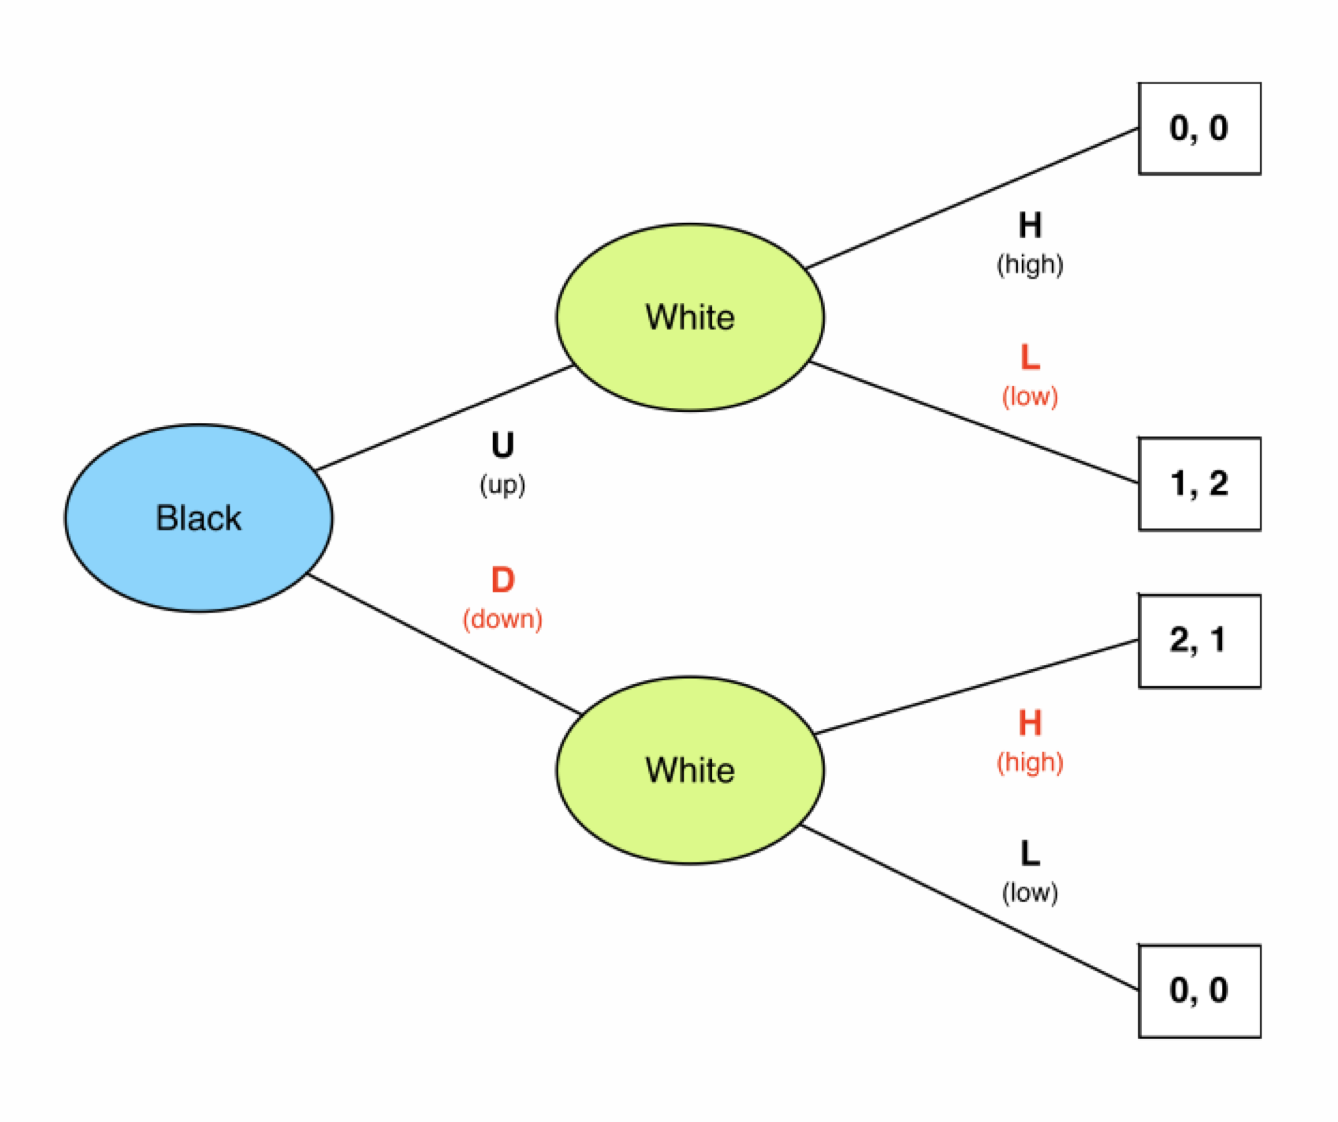
\includegraphics[width=0.6\textwidth]{img/01_sequential_games/gametree_backward_induction.png}
			\caption{Backward Induction am Beispiel eines simplen Spielbaums}
			\label{fig:01_seq_backward_induction}
		\end{figure}
	
		\begin{itemize}
			\item Backward Induction ist der Lösungsalgorithmus für endliche, sequenzielle Spiele
			\item Im Beispiel oben hat Black den First-Mover Vorteil.
			\item Wenn beide Spieler perfekt spielen, endet das Spiel mit den Payoffs (2,1) \\
				(2 für Black, 1 für White)
			\item Solche Spiele immer rückwärts analysieren!
		\end{itemize}
	
		\subsection{Reasoning about Finite Sequential Games}
		
		\begin{itemize}
			\item Eine \textbf{ultra-schwache Lösung} beweist ob der erste Spieler aus der Initialposition gewinnen, verlieren oder unentschieden machen wird, in Annahme eines perfekten Spiels des Gegners \\
			\textit{Im Beispiel: Schwarz kann einen Gewinn forcieren und hat demnach den First-Mover Vorteil}
			
			\item Eine \textbf{schwache Lösung} bietet einen Algorithmus welcher ein komplettes Spiel an perfekten Zügen aus der Initialposition offenbart, in Annahme eines perfekten Spiels des Gegners \\
			\textit{Schwache Lösung für das Spiel: Black spielt U, White spielt L, Black spielt D}
			
			\item Eine \textbf{starke Lösung} bietet einen Algorithmus, welcher perfekte Züge aus jeder Position produzieren kann, auch wenn vorher von irgendeinem Spieler Fehler gemacht wurden. \\
			\textit{Starke Lösung für dieses Spiel:}
				\begin{itemize}
					\item \textit{Algorithmus für White: wenn Black U spielt $\rightarrow$ spiel L; wenn Black D spielt $\rightarrow$ spiel H}
					\item \textit{Algorithmus für Black: Spiel D im ersten Zug; wenn White L im oberen Knoten spielt, spiel D}
				\end{itemize}
		\end{itemize}
	
		\paragraph{A Strong Solution to Nim}
		
		
		
		Algorithmus für einen perfekten Nim Bot:
		
		\begin{enumerate}
			\item Wenn nur ein Haufen übrig bleibt \\
				$\rightarrow$ Nimm alle Objekte des Haufens und hol den Preis
			\item Wenn zwei Haufen mit unterschiedlicher Anzahl Objekte übrig bleiben \\
				$\rightarrow$ Nimm Objekte vom grösseren Haufen und mache beide gleich gross
			\item Wenn zwei Haufen diesselbe Anzahl Objekte haben \\
				$\rightarrow$ Egal was du tust, du hast verloren (in Annahme eines perfekten Spiels des Gegners)
		\end{enumerate} 
	
		\newpage
	
		\subsection{Zero-Sum Games}
		
		\begin{itemize}
			\item Ein Spiel ist Zero-Sum, wenn der totale Gewinn des Siegers gleich dem totalen Verlust des Verlierers ist
				\begin{itemize}
					\item Einen Kuchen zu schneiden ist zero-sum bspw. wenn ich ein Stück esse, ist es für dich verloren
					\item Brettspiele sind zero-sum bspw. wenn der Sieger +1 erhält und der Verlierer -1
				\end{itemize}
			\item $u_{1}$ und $u_{2}$ umschreiben die Utility-Funktion von Spieler 1 und 2, somit ist für jedes Strategiepaar $s_{1}$ und $s_{2}$ von Spieler 1 und 2 und es gilt $u_{1}(s_{1}, s_{2}) + u_{2}(s_{1}, s_{2}) = 0$, dann lässt sich sagen: \\
			$$u_{1}(s_{1}, s_{2}) = -u_{2}(s_{1}, s_{2})$$
		\end{itemize}
	
		\paragraph{Backward Induction \& Minimax}
		
		\begin{itemize}
			\item Backward Induction ist die Lösungsstrategie für endliche Spiele mit perfekter Information
			\item Eine einzelne Durchführung von Backward Induction aus einem Startzustand offenbart eine schwache Lösung.
			Wenn Backward Induction dynamisch (während des Spiels) aus jedem Zustand ausgeführt werden kann, erhalten wir eine starke Lösung.
			\item Wenn das Spiel zusätzlich zero-sum ist, kann Backward Induction mit dem Minimax Algorithmus implementiert werden.
			Minimax wird oft für Zwei-Spieler-Spiele definiert, ist aber auch für mehr Spieler erweiterbar.
			\item Minimax erlaubt effizientes Pruning ("Ausästen") und nahtlose Integration von Heuristiken
			\item Hinweis: Backward Induction kann auch für Spiele genutzt werden, die nicht zero-sum sind und kompliziertere Payoffs enthalten als eine einzelne Zahl
		\end{itemize}
	
		\subsection{Minimax Algorithm}
		
		\begin{itemize}
			\item 1928 von John von Neumann erfunden
			\item Beide Spieler wollen ihre respektiven Payoffs maximieren
			\item Weil das Spiel zero-sum ist, ist mein Gewinn = Verlust des Gegners
			\item Anstatt nach eigenem Gewinn zu maximieren, kann der Gewinn des Gegeners minimiert werden
			\item Im Spielbaum kann folgendermassen vorgegangen werden:
				\begin{itemize}
					\item Gehört der Knoten mir, wähle die Aktion welche den Payoff maximiert
					\item Gehört der Knoten dem Gegner, wähle die Aktion welche den Payoff minimiert
				\end{itemize}
		\end{itemize}
	
		\begin{figure}[htb!]
			\centering
			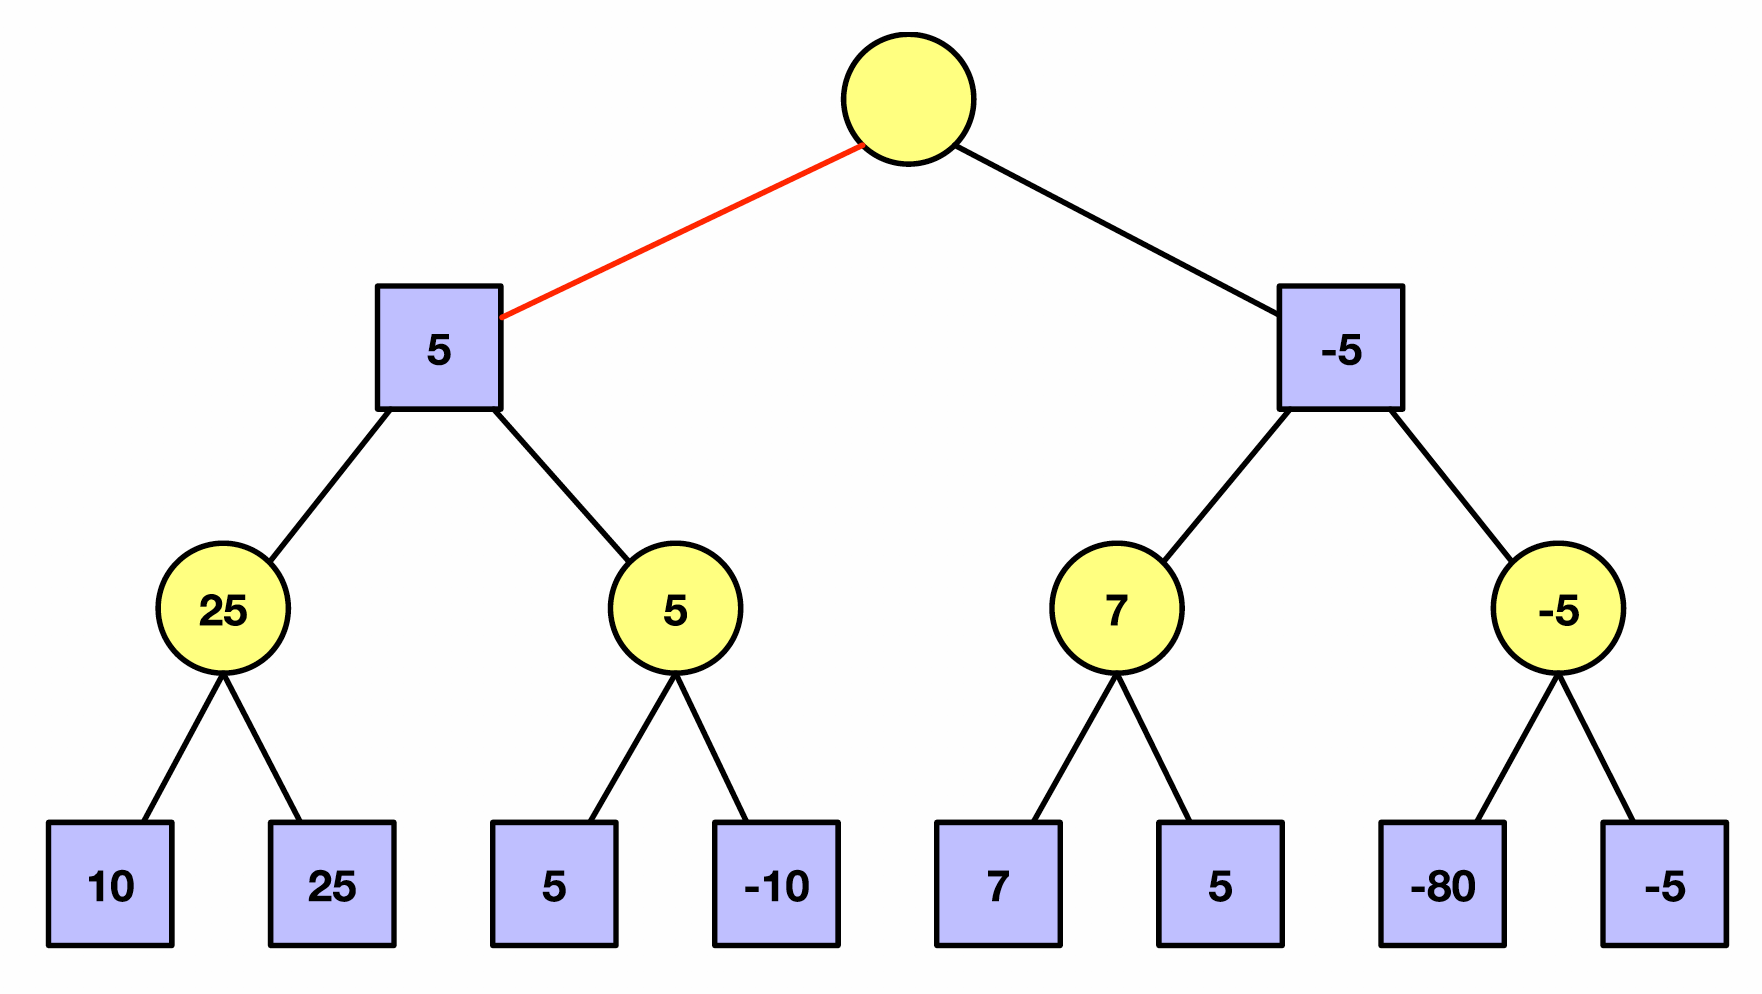
\includegraphics[width=0.6\textwidth]{img/01_sequential_games/minimax_solution.png}
			\caption{Lösungsweg eines Spielbaums mithilfe des Minimax-Algorithmus}
			\label{fig:01_seq_minimax_solution}
		\end{figure}
	
		\paragraph{Programming a Minimax Bot}
		
		\begin{itemize}
			\item Minimax implementiert Backward Induction für zero-sum Spiele.
				Dank der vereinfachenden zero-sum Eigenschaft können einige Tricks angewandt werden, um einen herusitischen Algorithmus zu erhalten:
			\begin{itemize}
				\item Minimax nur bis zu einer limitierten Tiefe, bspw. 5 Runden vorausschauen und dann stoppen.
					Wie tief man gehen kann ist abhängig von den Spielregeln (Anzahl mögliche Züge), Effizienz der Implementation und Rechenleistung.
				\item Da die Tiefe limitiert ist, werden die Blattknoten nicht erreicht und wir kennen die echten Payoffs nicht.
					Wir müssen eine Heuristik erfinden, um die Situation abzuschätzen an welcher wir stoppen.
					Je besser die Heuristik, desto besser der Bot.
			\end{itemize}
		\end{itemize}
	
		\begin{figure}[htb!]
			\centering
			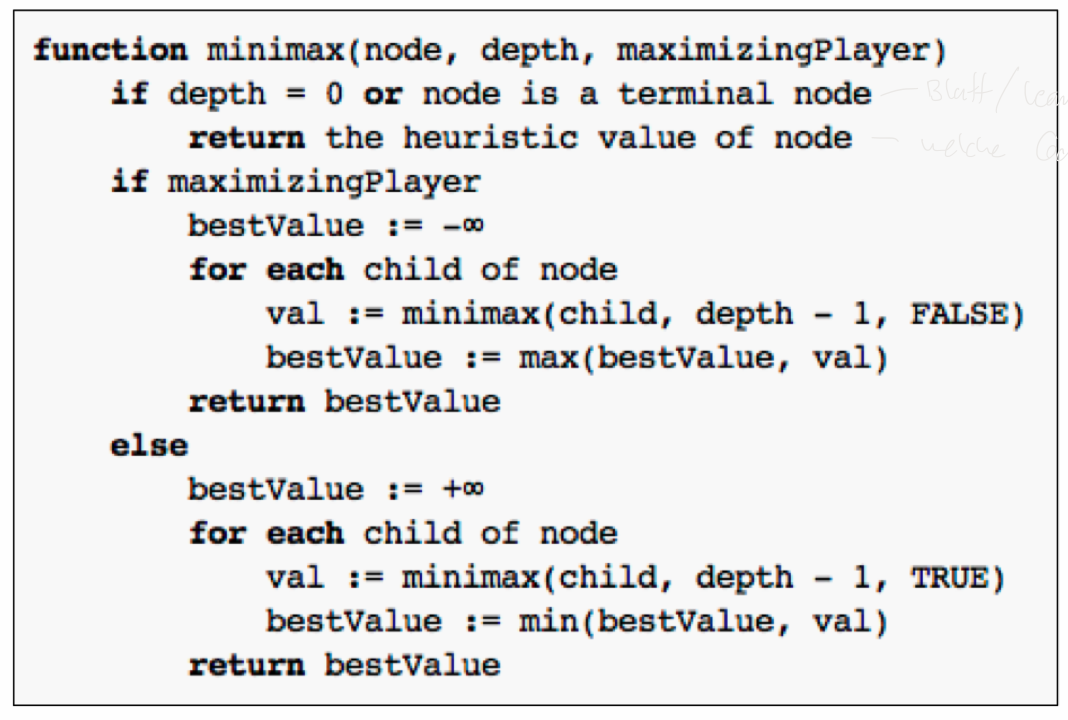
\includegraphics[width=0.6\textwidth]{img/01_sequential_games/minimax_pseudocode.png}
			\caption{Pseudocode eines Minimax-Algorithmus mit limitierter Tiefe und Heuristik}
			\label{fig:01_seq_minimax_pseudocode}
		\end{figure}
	
		\subsection{Search Tree Pruning}
		
		\begin{itemize}
			\item Es müssen nicht alle Knoten abgelaufen werden, um die optimale Strategie zu finden.
			\item Wir "stutzen" (prunen) Sub-Bäume, welche keine bessere Lösung beinhalten können und demnach nicht besucht werden müssen.
			\item Dazu enthält der Algorithmus zwei Parameter: \\
			\textit{(Vorfahren sind alle Knoten auf dem Weg zwischen dem aktuellen und dem Wurzelknoten)}
				\begin{itemize}
					\item $\alpha$ ist der höchste Wert aller MAX-Vorfahren eines MIN Knoten
					\item $\beta$ ist der tiefste Wert alles MIN-Vorfahren eines MAX Knoten
				\end{itemize}
			\item Der Algorithmus Alpha-Beta Pruning aktualisiert diese beiden Parameter im Minimax-Prozess und schneidet nicht besuchte Sub-Bäume ab, sobald er weiss dass die Werte aus diesem Sub-Baum den Wert $\alpha$ nicht überbieten oder $\beta$ nicht unterbieten können.
		\end{itemize}
		
		\paragraph{Alpha-Beta Pruning Rules}
		
		\begin{itemize}
			\item Alpha ($\alpha$) ist der minimale Score, welcher dem maximierenden Spieler versichert werden kann
			\item Beta ($\beta$) ist der maximale Score, welcher dem minimierenden Spieler versichert werden kann
			\item Daraus lassen sich folgende beiden Regeln schliessen:
				\begin{itemize}
					\item \textbf{Regel 1}: Schneide ab, sobald der aktuelle Wert eines MIN Knoten kleiner ist als $\alpha$
					\item \textbf{Regel 2}: Schneide ab, sobald der aktuelle Wert eines MAX Knoten grösser ist als $\beta$
				\end{itemize}
		\end{itemize}
	
		\subsection{Illustrations for Alpha-Beta Pruning}
		
		\begin{figure}[htb!]
			\centering
			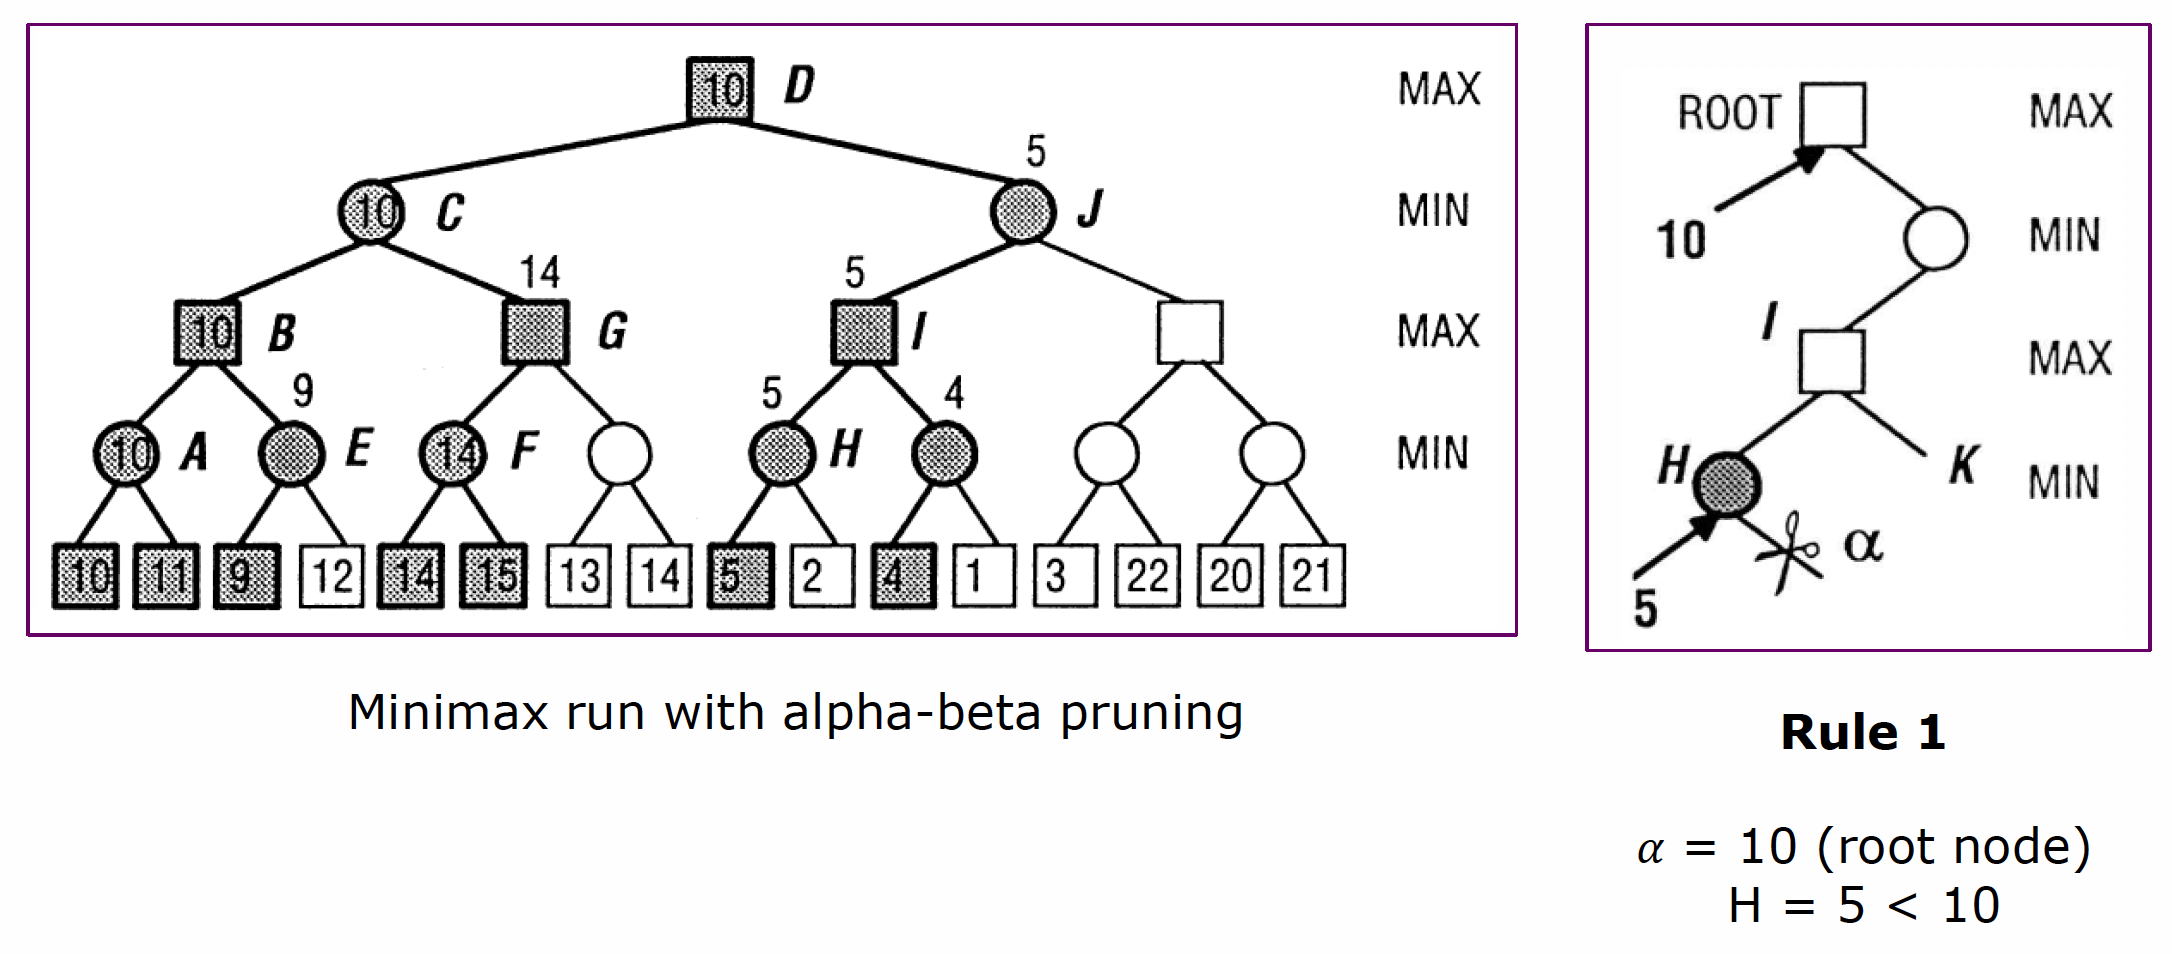
\includegraphics[width=0.5\textwidth]{img/01_sequential_games/alphabeta_rule1.png}
			\caption{Illustration der Durchführung der 1. Regel des Alpha-Beta Pruning}
			\label{fig:01_seq_alphabeta_rule1}
		\end{figure}
	
		\begin{figure}[htb!]
			\centering
			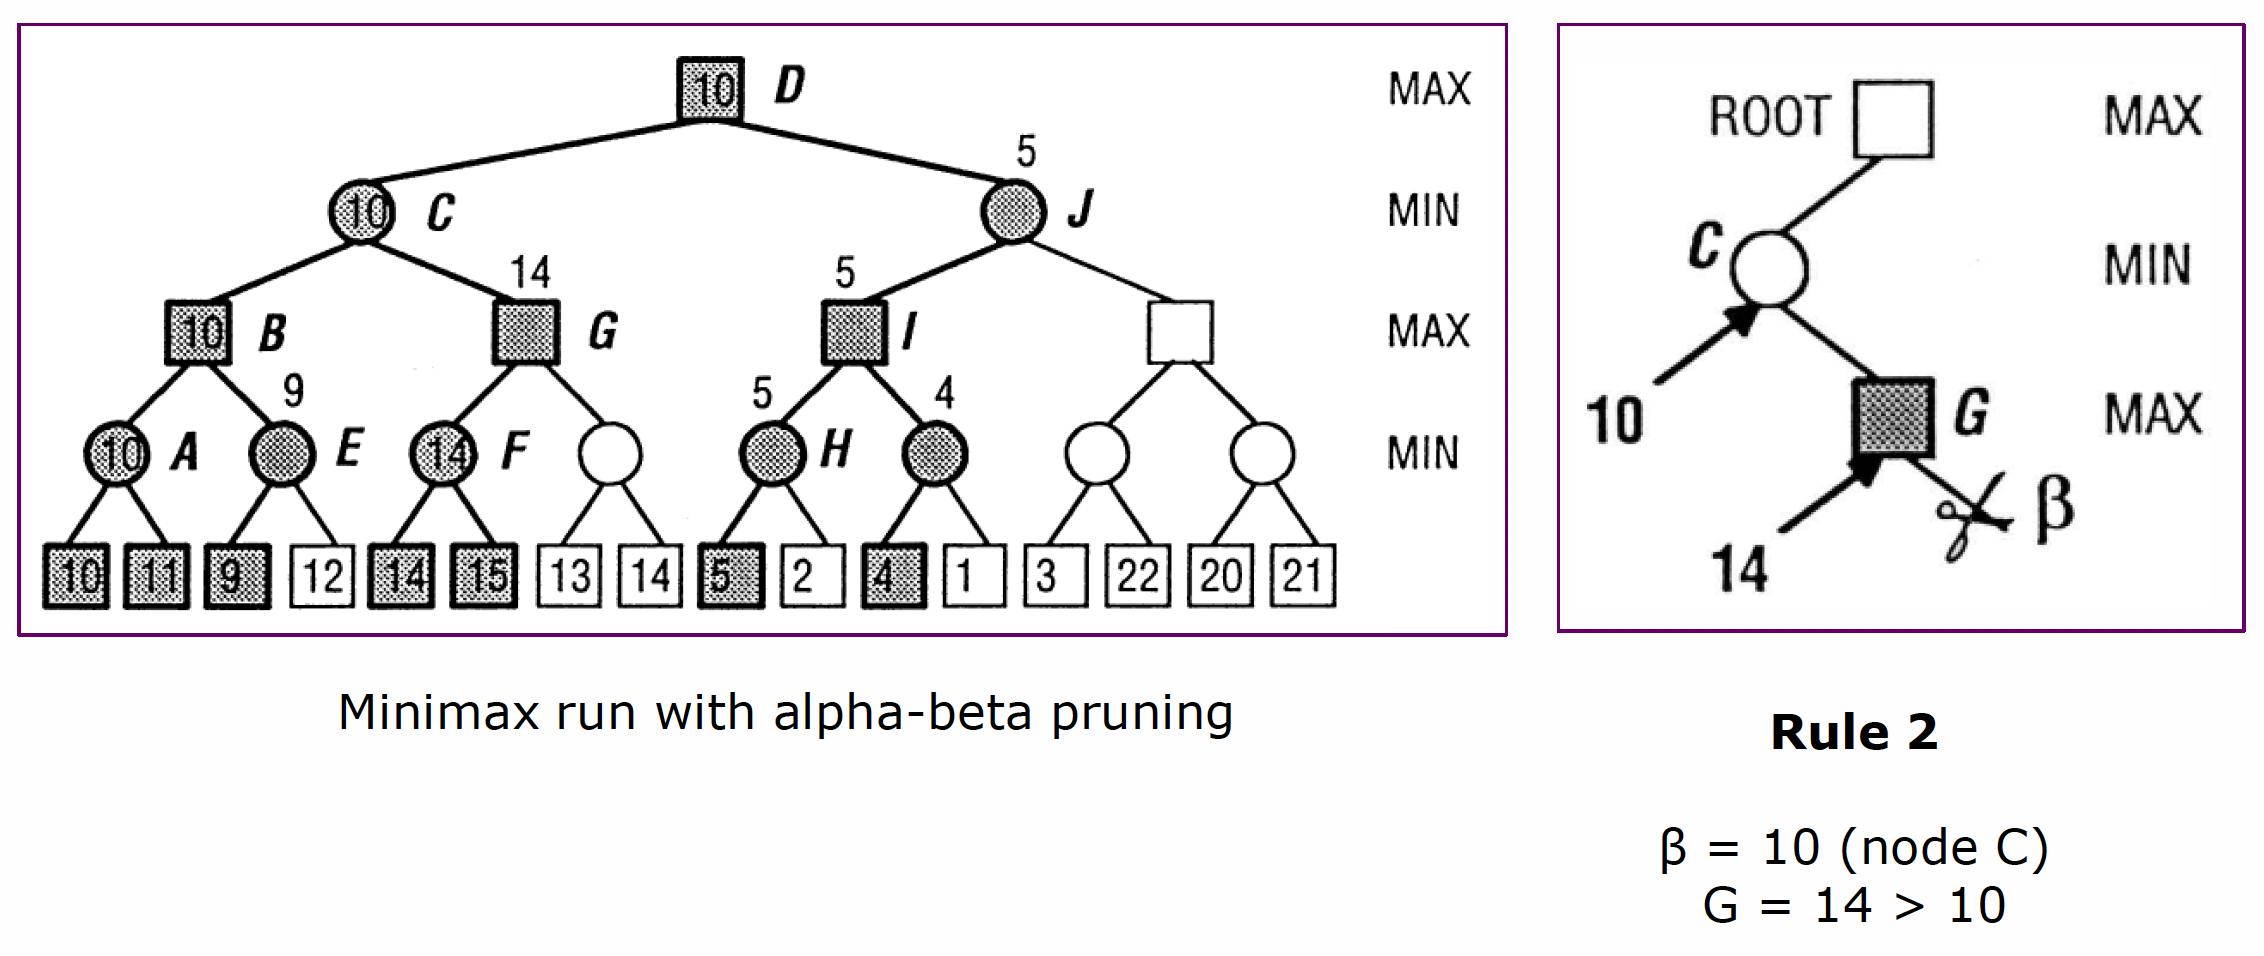
\includegraphics[width=0.5\textwidth]{img/01_sequential_games/alphabeta_rule2.png}
			\caption{Illustration der Durchführung der 2. Regel des Alpha-Beta Pruning}
			\label{fig:01_seq_alphabeta_rule2}
		\end{figure}
	
		\begin{figure}[htb!]
			\centering
			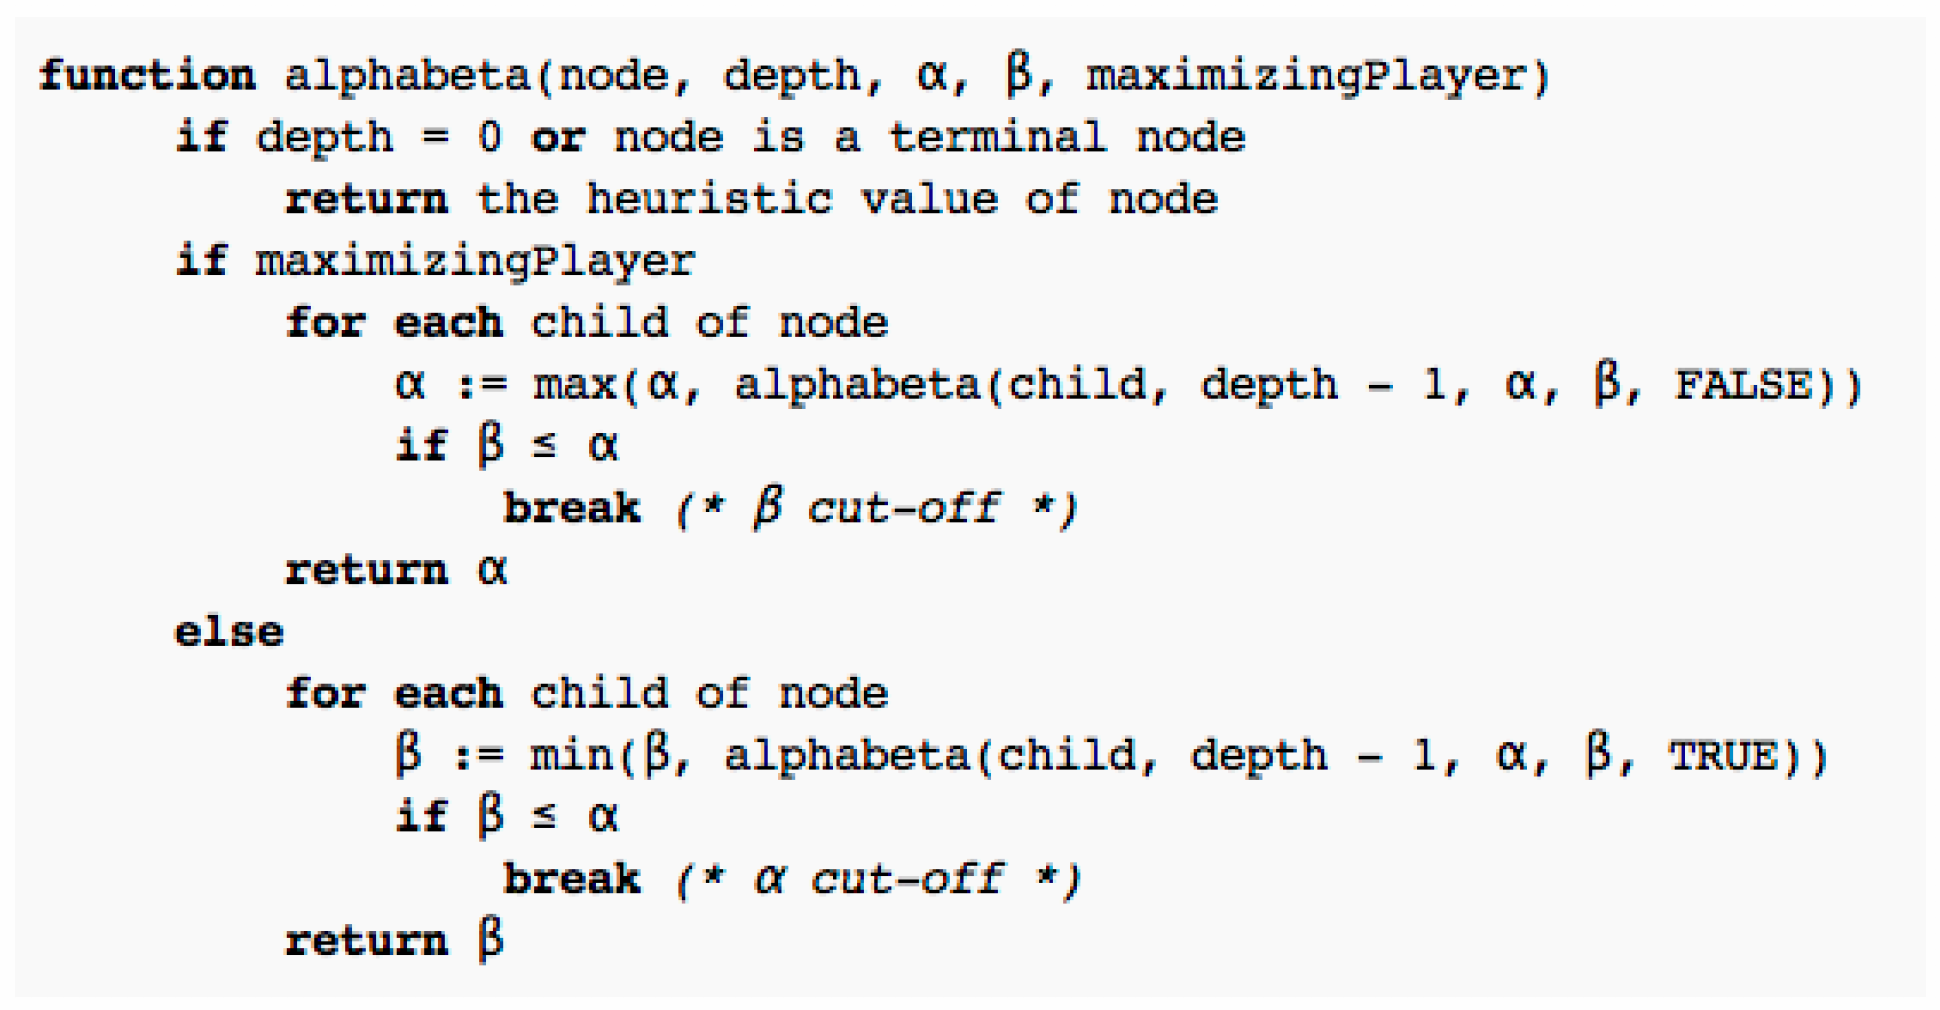
\includegraphics[width=0.5\textwidth]{img/01_sequential_games/alphabeta_pseudocode.png}
			\caption{Pseudocode eines Minimax mit limitierter Tiefe mithilfe von Alpha-Beta Pruning}
			\label{fig:01_seq_alphabeta_pseudocode}
		\end{figure}
	
		\paragraph{Speed-Up of Alpha-Beta Pruning}
		
		\begin{itemize}
			\item In einem Spielbaum mit Tiefe $m$ mit $b$ möglichen Aktionen bei jedem Knoten ist die Zeitkomplexität des Minimax O($b^{m}$) bzw.. es gibt b$^{m}$ Blattknoten
			\item Im Idealfall benötigt Alphe-Beta Pruning nur O($b^{m/2}$) = O($(\sqrt{b})^{m}$). 
			Dies korrespondiert zu einer Reduzierung des Branching-Faktors von $b$ zu $\sqrt{b}$, bspw. bei Schach bedeutet dies 6 mögliche Aktionen bei jedem Knoten (anstelle von 35)
			\item Um diesen maximalen Speed-Up zu erreichen, müssen die verschiedenen States in gescheiter Anordnung erforscht werden, was jedoch problemspezifisch ist.
		\end{itemize}
	
	\section{Monte Carlo Tree Search}
	
		\subsection{Random Walks}
		
		\begin{itemize}
			\item Suchräume sind meist zu gross für eine vollständige Suche
			\item Minimax soll bei einer bestimmten Baum-Tiefe stoppen und raten (mit Heuristik)
			\item Monte Carlo Tree Search ist ein anderes Vorgehen: \\
			\textit{Monte Carlo Tree Search führt Random Walks durch, um möglichst viel des Suchbaums in einem vorbestimmten Zeitraum abzusuchen.
			Danach wird der vielversprechendste Zug gespielt.}
		\end{itemize}
	
		\newpage
	
		\subsection{The 4 Phases in Monte Carlo Tree Search}
		
		\begin{enumerate}
			\item \textbf{Selection}
				\begin{itemize}
					\item Starte beim Wurzelknoten \texttt{R} und wähle fortlaufend Kinderknoten
					\item Stoppe, wenn du einen Knoten erreichst, der noch nicht komplett erweitert/erforscht wurde
					\item Benötigt ein Kriterum für die Auswahl der Kinderknoten, sogennante \textit{tree policy}
				\end{itemize}
			\item \textbf{Expansion}
				\begin{itemize}
					\item Wenn das Zeitlimit \texttt{L} das Spiel beendet, gib die Payoffs zurück
					\item Sonst, wähle eine unerforschte Aktion und kreiere einen Knoten \texttt{C} für diese
				\end{itemize}
			\item \textbf{Simulation}
				\begin{itemize}
					\item Simuliere ein Weiterspielen von Knoten \texttt{C} aus, mithilfe einer \textit{default policy}
					\item Im simpelsten Fall, spiele einfach bis zu irgendeinem Ende mit zufälligen Zügen
				\end{itemize}
			\item \textbf{Backpropagation}
				\begin{itemize}
					\item Aktualisiere die gespeicherten Informationen in jedem Knoten von \texttt{C} zurück bis zu \texttt{R}
					\item MCTS erwartet einen Payoff in [0,1]
				\end{itemize}
		\end{enumerate}
	
		\subsection{MCTS for Tic-Tac-Toe}
		
		\begin{figure}[htb!]
			\centering
			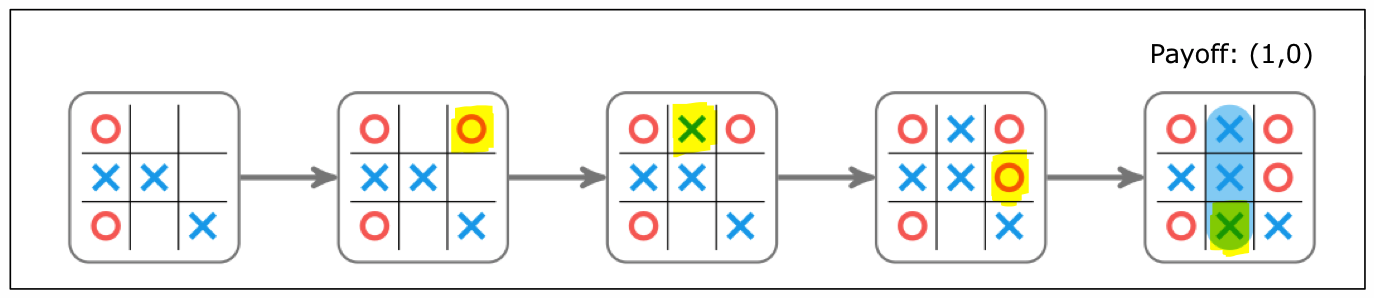
\includegraphics[width=0.6\textwidth]{img/02_mcts/random_ttt.png}
			\caption{Zufälliger Durchlauf eines Runde Tic-Tac-Toe}
			\label{fig:02_mcts_random_tictactoe}
		\end{figure}
	
		\begin{itemize}
			\item Es gibt Punkte für einen Gewinn (1), unenentschieden (0.5) und Verlust (0)
			\item MCTS ist nicht limitiert auf zero-sum Spiele
			\item Payoffs werden durch Vektoren repräsentiert
			\item Die Simulation endet mit einem Gewinn für Spieler X mit Payoff +1 $\rightarrow$ Payoff-Vektor (1,0) \\
			(Spieler Y hat in dieser Simulation also einen Payoff von 0)
		\end{itemize}
	
		\begin{figure}[htb!]
			\centering
			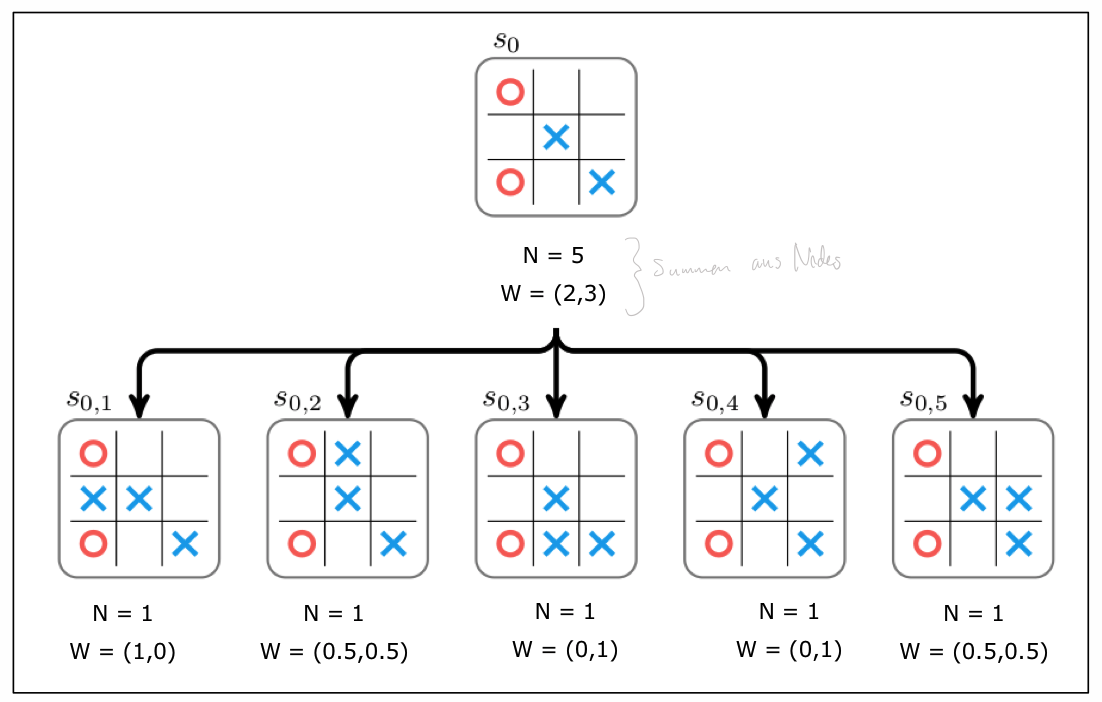
\includegraphics[width=0.6\textwidth]{img/02_mcts/ttt_payoffs.png}
			\caption{übersicht der Simulationen eines Tic-Tac-Toe Spiels}
			\label{fig:02_mcts_ttt_payoffs}
		\end{figure}
	
		\begin{itemize}
			\item \texttt{N} speichert die Anzahl Simulationen, die vom Knoten $s_{0}$ aus gestartet wurden
			\item \texttt{W} sind die akkumulierten Payoff-Vektoren (eine Komponente für jeden Spieler)
			\item Backpropagation kalkuliert lediglich die Summe von \texttt{N}$^{*}$ und \texttt{W}
			\item \textbf{Wichtig}: Ist der Wurzelknoten ebenfalls auch ein Kindesknoten, muss sein Payoff nach oben ebenfalls hinzugerechnet werden 
		\end{itemize}
	
		\newpage
	
		\subsection{Selection Policy: Which Node to Choose}
		
		\begin{figure}[htb!]
			\centering
			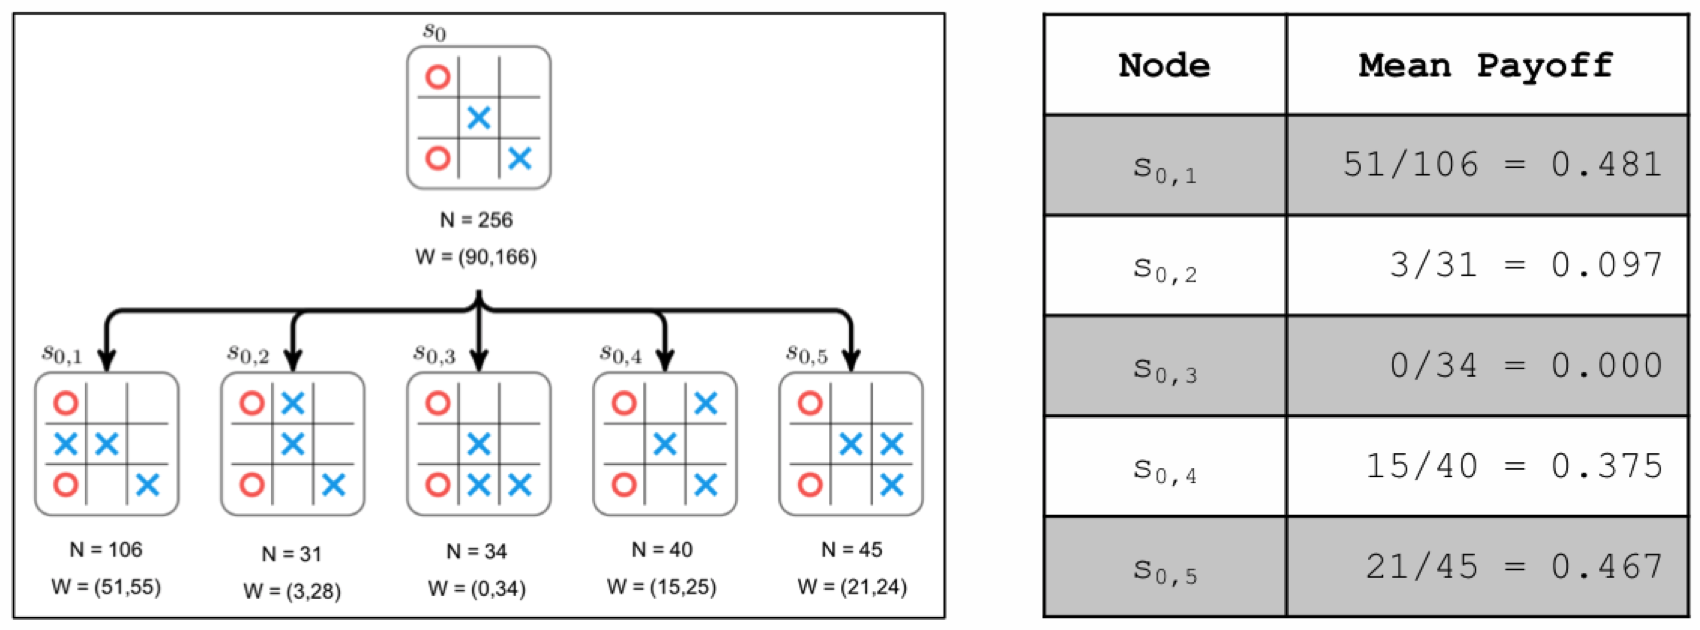
\includegraphics[width=0.8\textwidth]{img/02_mcts/selection_policy.png}
			\caption{Durchschnittliche Payoffs der durchlaufenen Simulationen mit MCTS}
			\label{fig:02_mcts_selection_policy}
		\end{figure}
		
		\begin{itemize}
			\item \textbf{Exploitation} \\
			Knoten $s_{0,1}$ hat den höchsten durchschnittlichen Payoff bzw. basierend auf aktuell verfügbaren Informationen, maximiert dieser Knoten meinen erwarteten Gewinn
			\item \textbf{Exploration} \\
			Knoten $s_{0,4}$ wurde nur 40 mal probiert, wie kann ich sicher sein dass der Score tiefer bleibt als bei $s_{0,1}$, auch wenn ich jetzt noch 66 mal spielen würde?
		\end{itemize}
	
		\subsection{Example of Multi-Armed Bandits}
		
		\begin{itemize}
			\item Es gibt eine Reihe an Slotmaschinen mit verschiedenen (unbekannten) Auszahlungswahrscheinlichkeiten und -mengen
			\item Man hat 1000 Münzen und möchte den erwarteten Gewinn erhöhen
			\item Idealerweise würde man immer an der Maschine mit dem grössten erwarteten Gewinn spielen
			\item Unglücklicherweise weiss man jedoch nicht, welche Maschine dafür am besten ist
			\item Es ist keine Person da, welcher man zuschauen und mehr über die Maschinen erfahren kann
		\end{itemize}
		\vspace{1em}
		Wie wählt man nun die beste Strategie in dieser Situation?
	
		\subsection{UCB1: Upper Confidence Bound}
		
		\begin{itemize}
			\item Am besten Exploration und Exploitation ausbalancieren
				\begin{itemize}
					\item \textbf{Exploration}: Spiele alle Maschinen um möglichst viele Informationen zu sammeln
					\item \textbf{Exploitation}: Spiele die beobachtet beste Maschine um den erwarteten Gewinn zu maximieren
				\end{itemize}
			\item UCB1 bietet die beste Balance zwischen Exploration und Exploitation, es gibt quasi ein statistisches Konfidenzintervall für jede Maschine aus
				\begin{itemize}
					\item Parameter $c \geq 0$ kontrolliert den Trade-Off zwischen Exploitation (tiefes $c$) und Exploration (hohes $c$)
				\end{itemize}
		\end{itemize}
	
		$$U_{i} = \frac{W_{i}}{N_{i}} + c \sqrt{\frac{\ln N_{p}}{N_{i}}}$$
		
		\vspace{1em}
		\begin{description}
			\item[$\frac{W_{i}}{N_{i}}$] \textbf{Exploitation}, der durchsch. Gewinn für Maschine $i$ ($\frac{W(Gewinne)}{N(Versuche)}$)
			\item
			\item[$\sqrt{\frac{\ln N_{p}}{N_{i}}}$] \textbf{Exploration}
				\begin{description}
					\item[$N_{p}$] Wie oft haben wir insgesamt gespielt (wie viele Münzen wurden verbraucht)
					\item[$N_{i}$] Wie oft wurde Maschine $i$ ausprobiert
				\end{description}
		\end{description}
		
		\newpage
		
		\paragraph{How to play with UCB1}
		Für jede der 1000 Münzen...
		\begin{itemize}
			\item Kalkuliere das UCB1 ($U_{i}$) von jeder Maschine $i$
			\item Spiele an der Maschine mit dem höchsten Upper Bound ($U_{i}$)
			\item Wähle entweder zufällig oder in numerischer Ordnung
			\item Solange man dies tut, wird der beobachtete Mittelwert für die Maschine sich verschieben und das Konfidenzintervall wird schmaler, aber die Intervalle aller anderen Maschinen werden breiter.
			Der Upper Bound einer anderen Maschine wird womöglich grösser als jener der aktuellen Maschine und man wird zu dieser Maschine wechseln.
			\item Bei Berechnung des UCB1 muss die Vektorkomponente für den aktuellen Spieler gewählt werden! \\
				Bsp. UCB1($s_{0,1}$) = 0.71, UCB1($s_{0,2}$) = ...
		\end{itemize}
	
		\paragraph{The final Move}
		
		\begin{itemize}
			\item Wenn die Zeit vorüber ist, spiele die erste Aktion mit der \textbf{höchsten Anzahl an Besuchen }$N$!
			\begin{itemize}
				\item Es benötigt keine Exploration wenn die finale Aktion ausgewählt werden soll
				\item Deshalb ist die Aktion mit dem höchsten UCB1 Score in der letzten Runde nicht zwingend die beste Wahl
				\item Die Aktion, welche am meisten gewählt wurde, gab meistens auch den höchsten UCB1 Score
			\end{itemize} 
		\end{itemize}
		
		\subsection{Minimax vs. Monte Carlo Tree Search}
		
		\begin{itemize}
			\item Beide Algorithmen setzen perfekte Information voraus
			\item Minimax ist nur für 2-Spieler zero-sum Spiele anwendbar
			\item MCTS funktioniert für jedes perfekte-Informationsspiel
			\item Minimax optimiert Payoffs; MCTS optimiert einen Exploitation-Exploration Trade-Off
			\item In Kontrast zu Minimax, ist MCTS ein "Anytime" Algorithmus
			\item Monte Carlo Bäume sind asymmetrisch, Minimax Bäume sind symmetrisch
		\end{itemize}
	
		\subsection{MCTS for Zero-Sum Games}
		
		\begin{itemize}
			\item Im Fall von 2 Spielern, Payoff Vektoren sind von der Form ($W, N-W$)
			\item Spieler 1 maximiert $W$, Spieler 2 maximiert $N-W$ (ignoriert den Exploitation-Teil in UCB1)
			\item Anders gesagt, könnte Spieler 2 $-W$ minimieren
			\item Wir können nur die Rewards $W$ für Spieler 1 speichern und die Zeichen für Spieler 2 "flippen"
			\item Daraus entsteht eine Minimax-ähnliche Variante von MCTS
		\end{itemize}
	
		\paragraph{Convergence to Optimal Play}
		
		\begin{itemize}
			\item Mit genügend Ressourcen konvergiert MCTS zu Minimax
			\item UCB1 hat logarithmisches Bereuen (\textit{logarithmic regret}), weil nur bestimmte Zeit zur Verfügung steht
			\item Die Fehlerwahrscheinlichkeit an der Wurzel des Baums konvergiert zu null in polynomialer Rate wenn die Anzahl simulierter Spiele in Richtung unendlich ansteigt.
			Dieser Beweist bedeutet, unter Annahme von genug Zeit, dass UCB1 der MCTS erlaubt zum Minimax-Baum zu konvergieren und ist demnach optimal.
		\end{itemize}
		
	\newpage	
	
	\section{Information Sets}
	
	\begin{figure}[htb!]
		\centering
		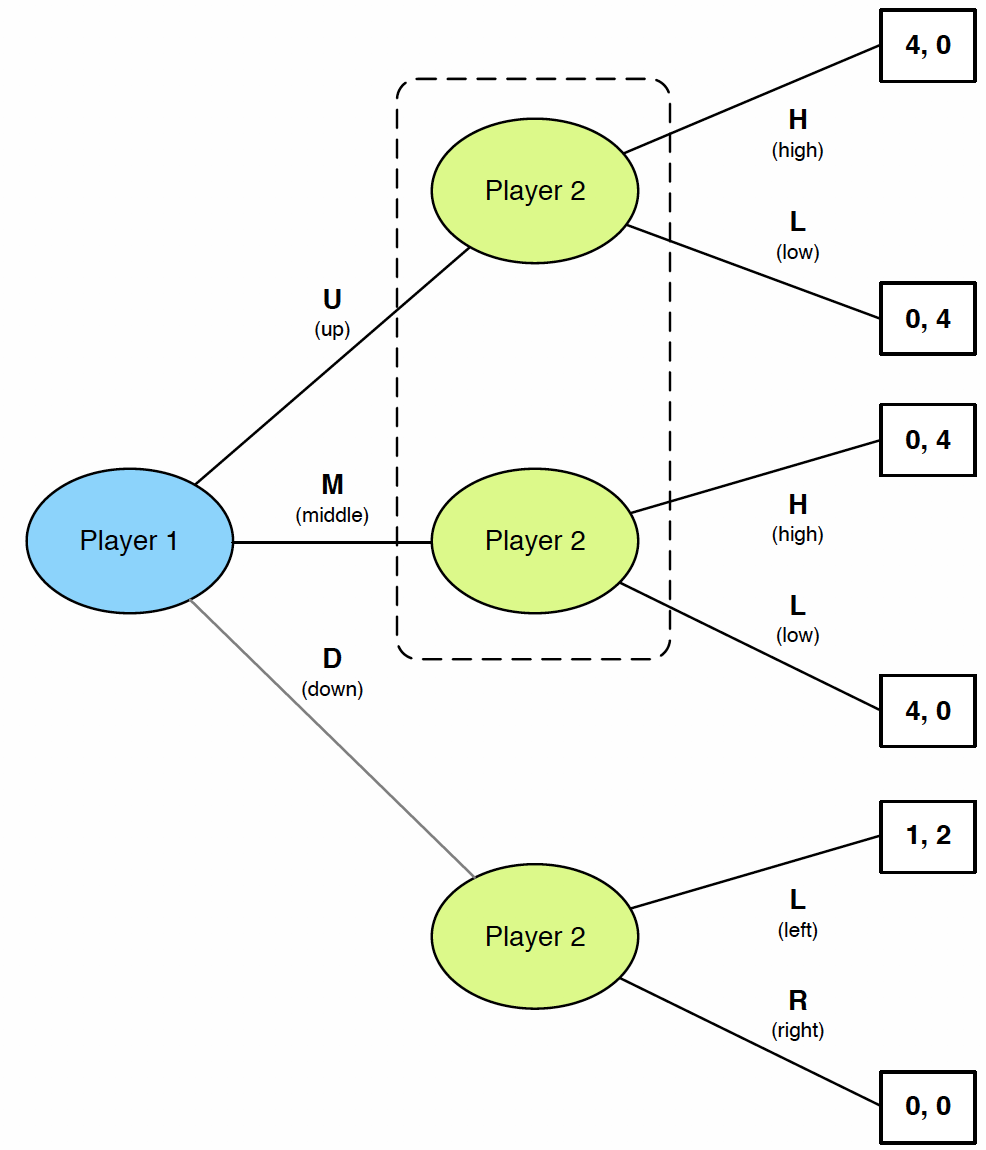
\includegraphics[width=0.4\textwidth]{img/03_information_sets/information_sets.png}
		\caption{Spielbeispiel mit imperfekter Information für Spieler 2}
		\label{fig:03_infosets_information_sets}
	\end{figure}

	\begin{itemize}
		\item In diesem Beispiel kann Spieler 2 nicht zwischen den oberen beiden Zuständen unterscheiden (gestrichelte Box),
			also ob Spieler 1 im ersten Zug U oder M gewählt hat.
		\item Er weiss also auch nicht, ob Spieler 1 D gewählt hat oder nicht
		\item Spieler 1 kann also zufällig zwischen U und M wählen
	\end{itemize}

		\subsection{Formal Definition of Information Sets}
		
		\begin{itemize}
			\item Ein Information Set von Spieler $i$ ist eine Sammlung von Knoten, welche Spieler $i$ gehören, zwischen welchen ich nicht unterscheiden kann.
			\item Es müssen einige Regeln erhoben werden, wie ein Information Set aufgebaut sein sollen.
				Ansonsten könnte Spieler 2 betrügen (bspw. mithilfe von Side-Channel-Informationen).
				Wir gehen jedoch von Perfect Recall aus, dass sich jeder Spieler seine bisherigen Züge merken kann.
				\begin{enumerate}
					\item Alle Knoten in einem Information Set müssen die gleichen Aktionen / Kinder haben.
					\item Aufgrund meiner Historie (bzw. vorgängigen Aktionen) darf ich keinen Hinweis darauf erhalten, dass ich mich in einem Information Set befinde.
				\end{enumerate}
		\end{itemize}
	
		\subsection{Perfect vs. Imperfect Information}
		
		\begin{itemize}
			\item In einem perfekten Informaionsspiel besteht jedes Information Set aus genau einem Knoten.
				Ansonsten ist es ein Spiel mit imperfekter Information.
			\item Eine (pure) Strategie von Spieler $i$ ist ein kompletter Plan von Aktionen.
				Sie spezifiziert, was Spieler $i$ tun wird, für jedes seiner Information Sets.
			\item Backward Induction kann nicht für Spiele mit imperfekter Information angewandt werden
			\item Stattdessen müssen sequenzielle Spiele mit imperfekter Information in simultane Spiele umgewandelt und mit der Best Response Funktion ein Gleichgewicht gefunden werden.
		\end{itemize}
	
		\subsection{Determinization}
		
		\begin{itemize}
			\item Determinization erlaubt, alle Möglichkeiten für Spiele mit perfekter Information für Spiele mit imperfekter Information nutzen zu können.
			\item Eine Determinization ist eine Probe aus dem Information Set des aktuellen Spielstands, bspw. für Kartenspiele, ziehe zufällig eine Handvoll Karten an Spieler, welche konsistent ist mit den Beobachtungen des aktuellen Spielers
			\item Zum Beispiel:
				\begin{itemize}
					\item Wende MCTS auf jede Determinization an
					\item Wähle einen Zug, für welchen die summierte Anzahl Besuche über alle Bäume hinweg maximal ist
				\end{itemize}
		\end{itemize}
	
		\subsection{Strategy Fusion}
		
		Strategy Fusion referenziert auf den Effekt, wenn ein deterministischer "Solver" unterschiedliche Entscheidungen innerhalt desselben Information Set macht
		
			\subsubsection{Strategy Fusion Example}
			
			\begin{figure}[htb!]
				\centering
				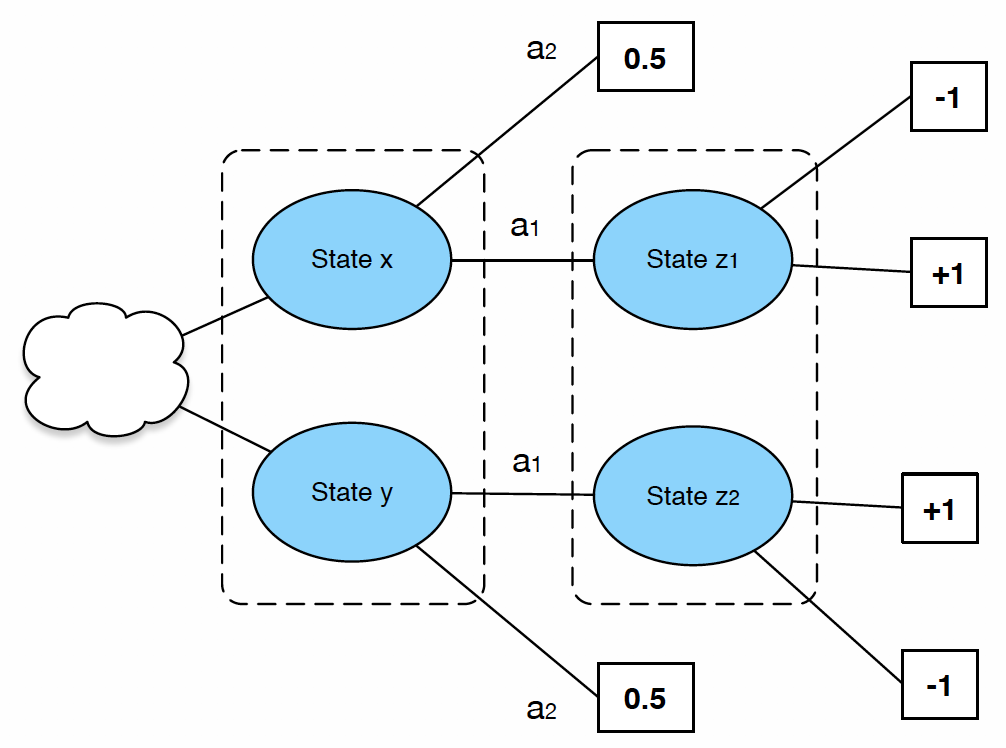
\includegraphics[width=0.5\textwidth]{img/03_information_sets/strategy_fusion.png}
				\caption{Strategy Fusion an einem Information Set Beispiel}
				\label{fig:03_infoset_strategy_fusion}
			\end{figure}
		
			\begin{itemize}
				\item 1-Spieler-Spiel mit zwei Information Sets
				\item Spieler kann $a_{2}$ wählen für einen sofortigen Payoff von 0.5
				\item Wählt er $a_{1}$, ist der erwartete Payoff 0
				\item Die beste Strategie ist demnach $a_{2}$ zu spielen
				\item Determinization würde von {x,y} sampeln und einen perfekten-Informations-Gewinn spielen
				\item Aber Sampling vom ersten Information Set würde das zweite Information Set auflösen (unter Annahme von Perfect Recall)
				\item In einem perfekten Informationsspiel würde der Spieler bei der Wahl von $a_{1}$ immer einen Payoff von +1 erhalten
				\item Determinization würde hier fälschlicherweise empfehlen, $a_{1}$ zu spielen
				\item Dies rührt daher, dass wir mit perfekter Information den besten Spielzug von $z_{1}$ und $z_{2}$ bestimmen könnten
			\end{itemize}
		
		\subsection{Information Set Search Trees}

		Strategy Fusion bewältigen, indem ein Baum von Information Sets durchsucht wird, anstelle von Zuständen.
		(Sampling von {x,y} enthüllt nicht direkt $z_{1}$ oder $z_{2}$)

		\begin{figure}[htb!]
			\centering
			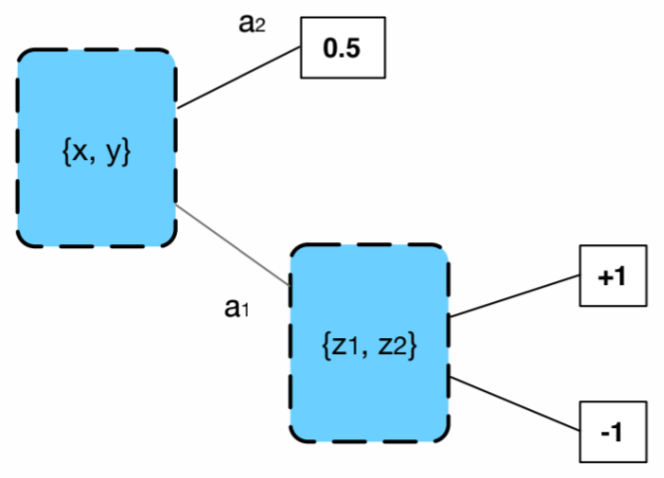
\includegraphics[width=0.3\textwidth]{img/03_information_sets/infoset_search_tree.png}
			\caption{Baum von Information Sets zur Durchsuchung}
			\label{fig:03_infoset_infoset_search_tree}
		\end{figure}
	
		\begin{figure}[htb!]
			\centering
			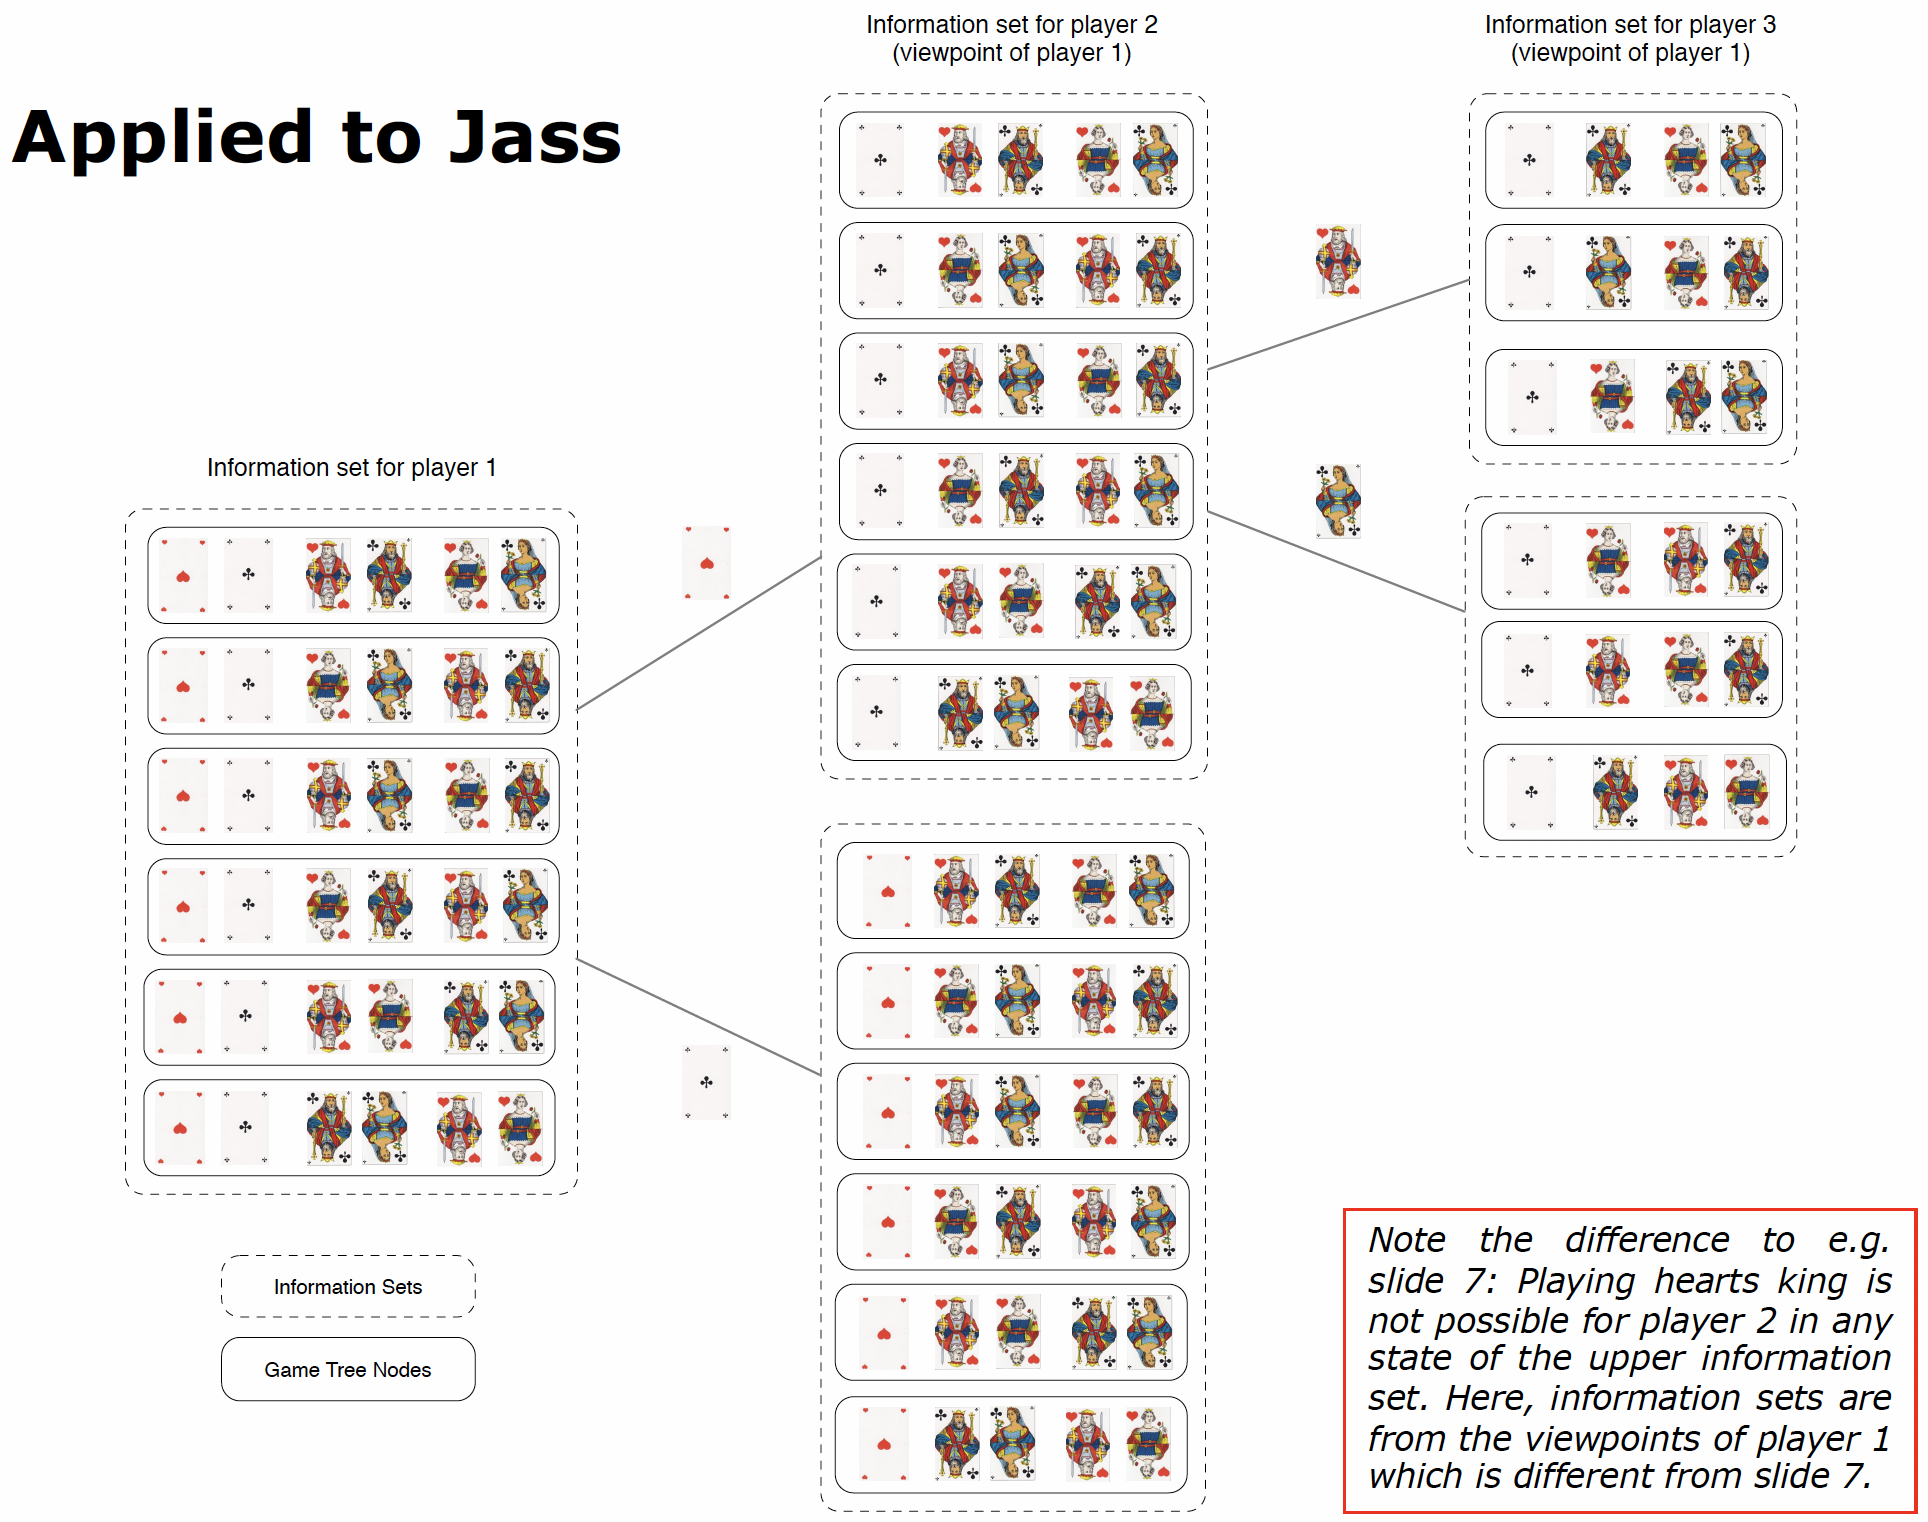
\includegraphics[width=0.8\textwidth]{img/03_information_sets/jass_search_tree.png}
			\caption{Information Set Search Trees am Beispiel von Jass}
			\label{fig:03_infoset_jass_search_tree}
		\end{figure}
	
		\subsection{Information Set Monte Carlo Tree Search}
		
		\begin{itemize}
			\item Knoten korrespondieren zu Information Sets aus der Sicht des Root-Spielers
			\item Kanten korrepondieren zu Aktionen (welche in mindestens einem Zustand verfügbar sind)
			\item Der Algorithmus beginnt damit, vom Root Information Set zu samplen und blendet alle inkompatiblen Knoten mit der gesampleten Determinization aus
			\item Dann wird MCTS auf dem perfekten Informationsspiel ausgeführt
		\end{itemize}
	
		\begin{figure}[htb!]
			\centering
			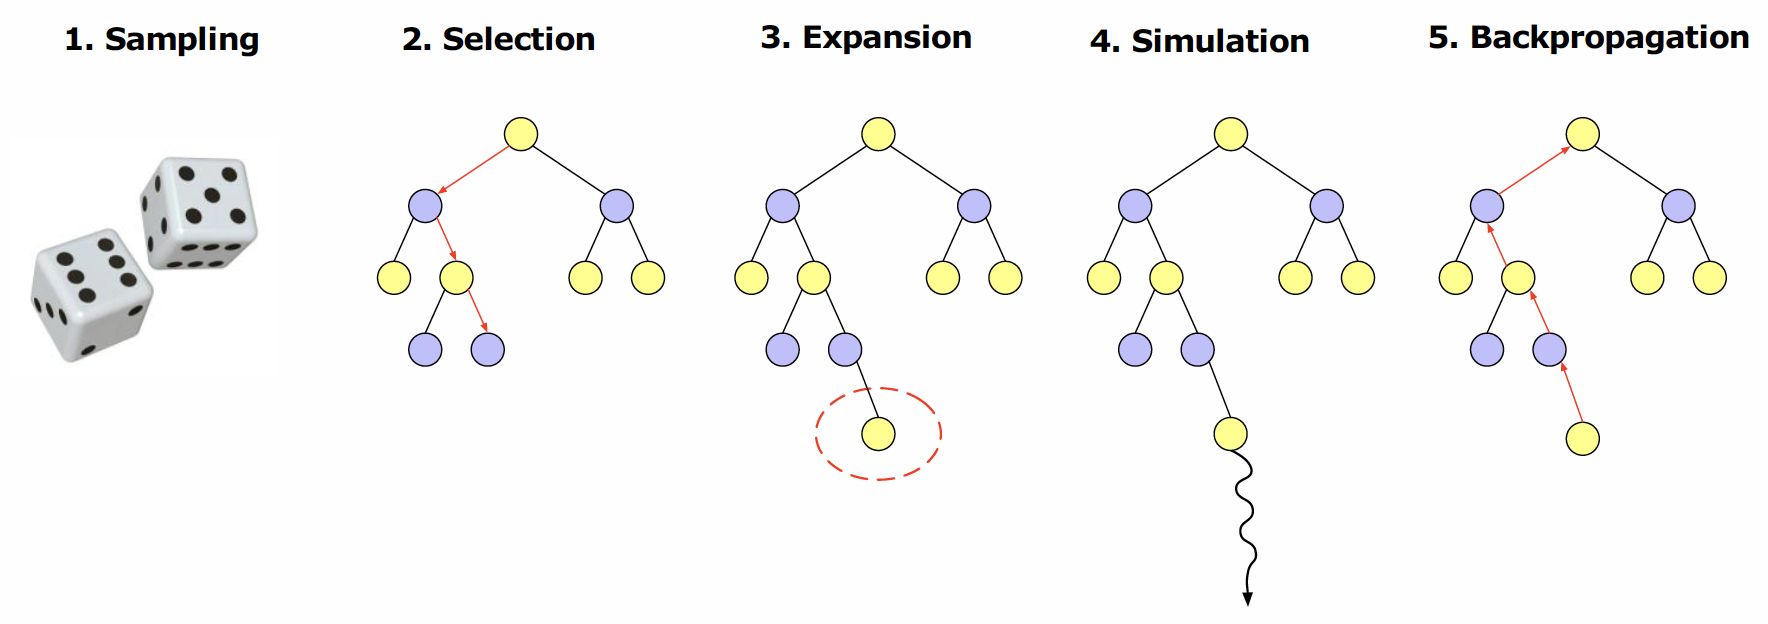
\includegraphics[width=0.8\textwidth]{img/03_information_sets/ismcts.png}
			\caption{Phasen der Information Set Monte Carlo Tree Search}
			\label{fig:03_infoset_ismcts}
		\end{figure}
	
		\newpage
	
		\paragraph{Necessary Change in Selection Phase}
	
		\begin{itemize}
			\item Für die Selection wird UCB1 verwendet:
			
			$U_{i} = \frac{W_{i}}{N_{i}} + c \sqrt{\frac{\ln N_{p}}{N_{i}}}$
			
			\item Bei ISMCTS kann sich die Anzahl möglicher Züge an einem gegnerischen Knoten zwischen den Besuchen an diesem Knoten unterscheiden
			\item Dies korrespondiert zum Subset-Armed-Bandit-Problem: \\
			Ersetze $N_{p}$ mit der Anzahl Besuchen des Vater-Knotens und wie oft Knoten $i$ verfügbar war für die Selection
			\item Ohne diese Modifizierung $\uparrow$ werden seltene Züge "übererforscht"
		\end{itemize}
	
		\subsection{Information Set vs. Perfect Information MCTS}
		
		\begin{itemize}
			\item ISMCTS hat den Vorteil, dass ganze "rechnerische Budget" auf einen einzelnen Baum konzentriert wird.
			Die Determinization-Technik hingegen teilt dies auf mehrere Bäume auf.
			Dies erlaubt üblicherweise eine tiefere Suche.
			\item Jedoch kann für einige Spiele, der Branching Faktor drastisch steigen aufgrund einer hohen Anzahl möglicher Züge bei jedem Information Set.
			Dadurch sinkt die Performance von ISMCTS in den meisten Fällen im Vergleich zur Determinization.
		\end{itemize}
	
	\section{Supervised Machine Learning}
	
		\subsection{Disciplines in Machine Learning}
		
		\begin{enumerate}
			\item Supervised Learning
				\begin{itemize}
					\item Dem Algorithmus werden gelabelte Trainingsdaten übergeben
					\item Er lernt, Labels von bisher unbekannten Beispielen voraussagen zu können
				\end{itemize}
			\item Unsupervised Learning
				\begin{itemize}
					\item Dem Algorithmus werden ungelabelte Daten übergeben
					\item Er erkennt und exploitiert die Struktur der Daten
				\end{itemize}
			\item Semi-Supervised Learning
				\begin{itemize}
					\item Eine Mischung aus supervised und unsupervised ML-Techniken
					\item Wird meist dann genutzt, wenn nur limitiert gelabelte Daten vorhanden sind
				\end{itemize}
			\item Reinforcement Learning
				\begin{itemize}
					\item Keine Daten verfügbar, aber der Algorithmus wird von einer Reward Funktion geleitet
					\item Es sucht das ideale Verhalten, welches den Reward des Agents maximiert
				\end{itemize}
		\end{enumerate}
	
		\subsection{Example Binary Classification Problem}
		
		\begin{figure}[htb!]
			\centering
			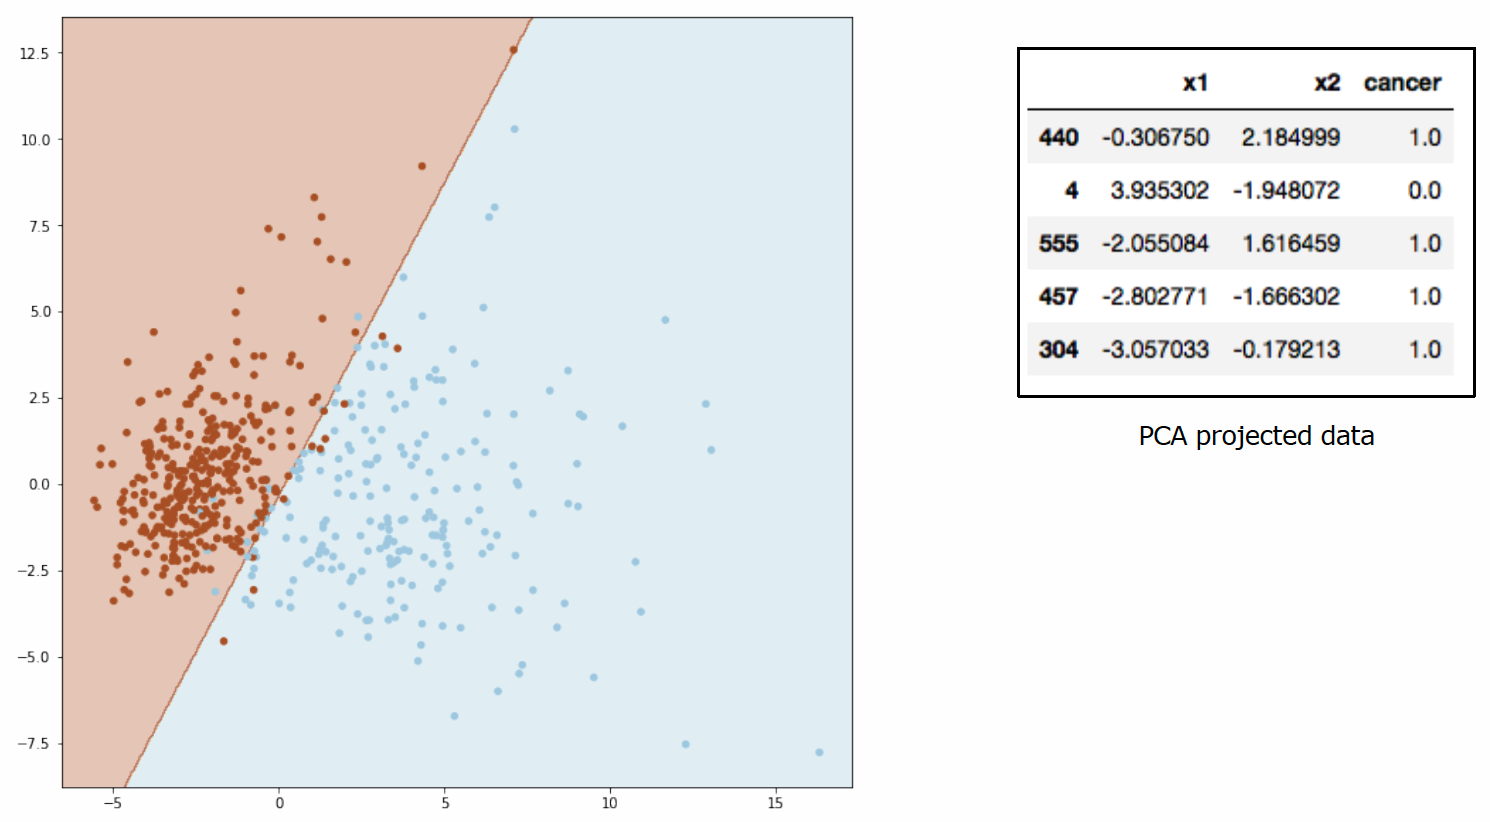
\includegraphics[width=0.7\textwidth]{img/04_supervised_ml/example_decision_boundary.png}
			\caption{Decision Boundary am Beispiel von Brustkrebsanalysen}
			\label{fig:04_superv_ml_example_decision_boundary}
		\end{figure}
	
		\newpage
	
		\begin{figure}[htb!]
			\centering
			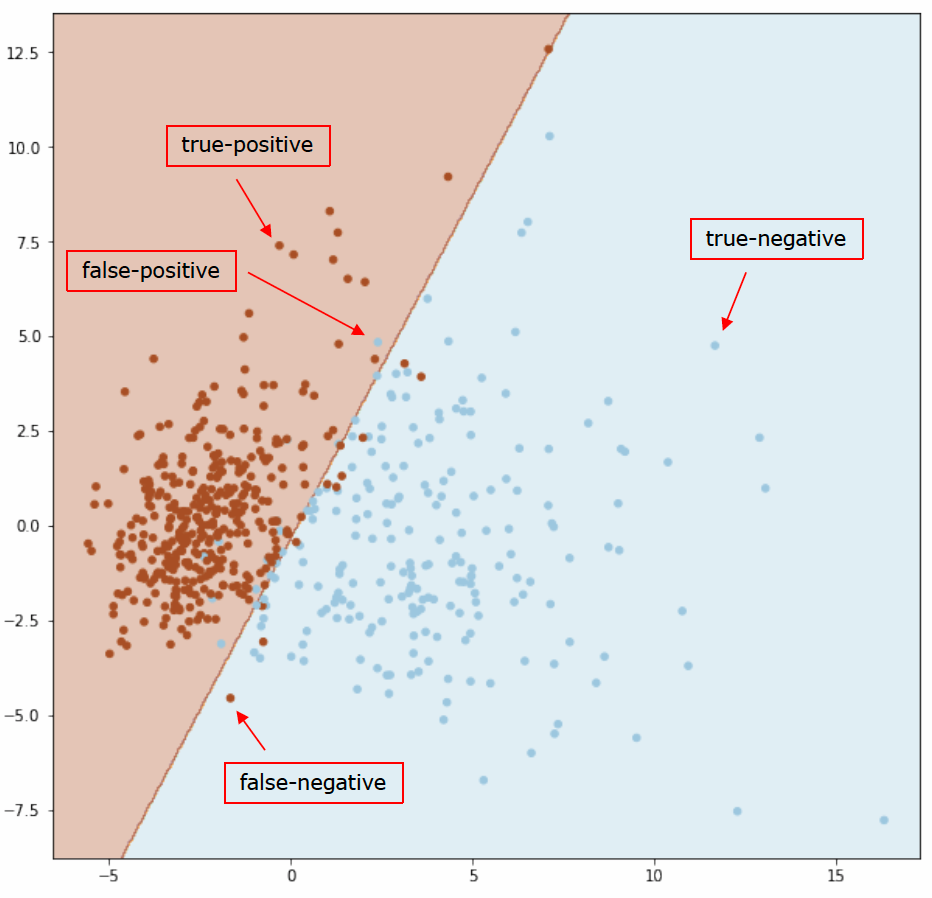
\includegraphics[width=0.6\textwidth]{img/04_supervised_ml/example_confusion_matrix.png}
			\caption{Beispiel der Confusion Matrix an Beispiel aus Abbildung \ref{fig:04_superv_ml_example_decision_boundary}}
			\label{fig:04_superv_ml_example_confusion_matrix}
		\end{figure}
	
		\begin{figure}[htb!]
			\centering
			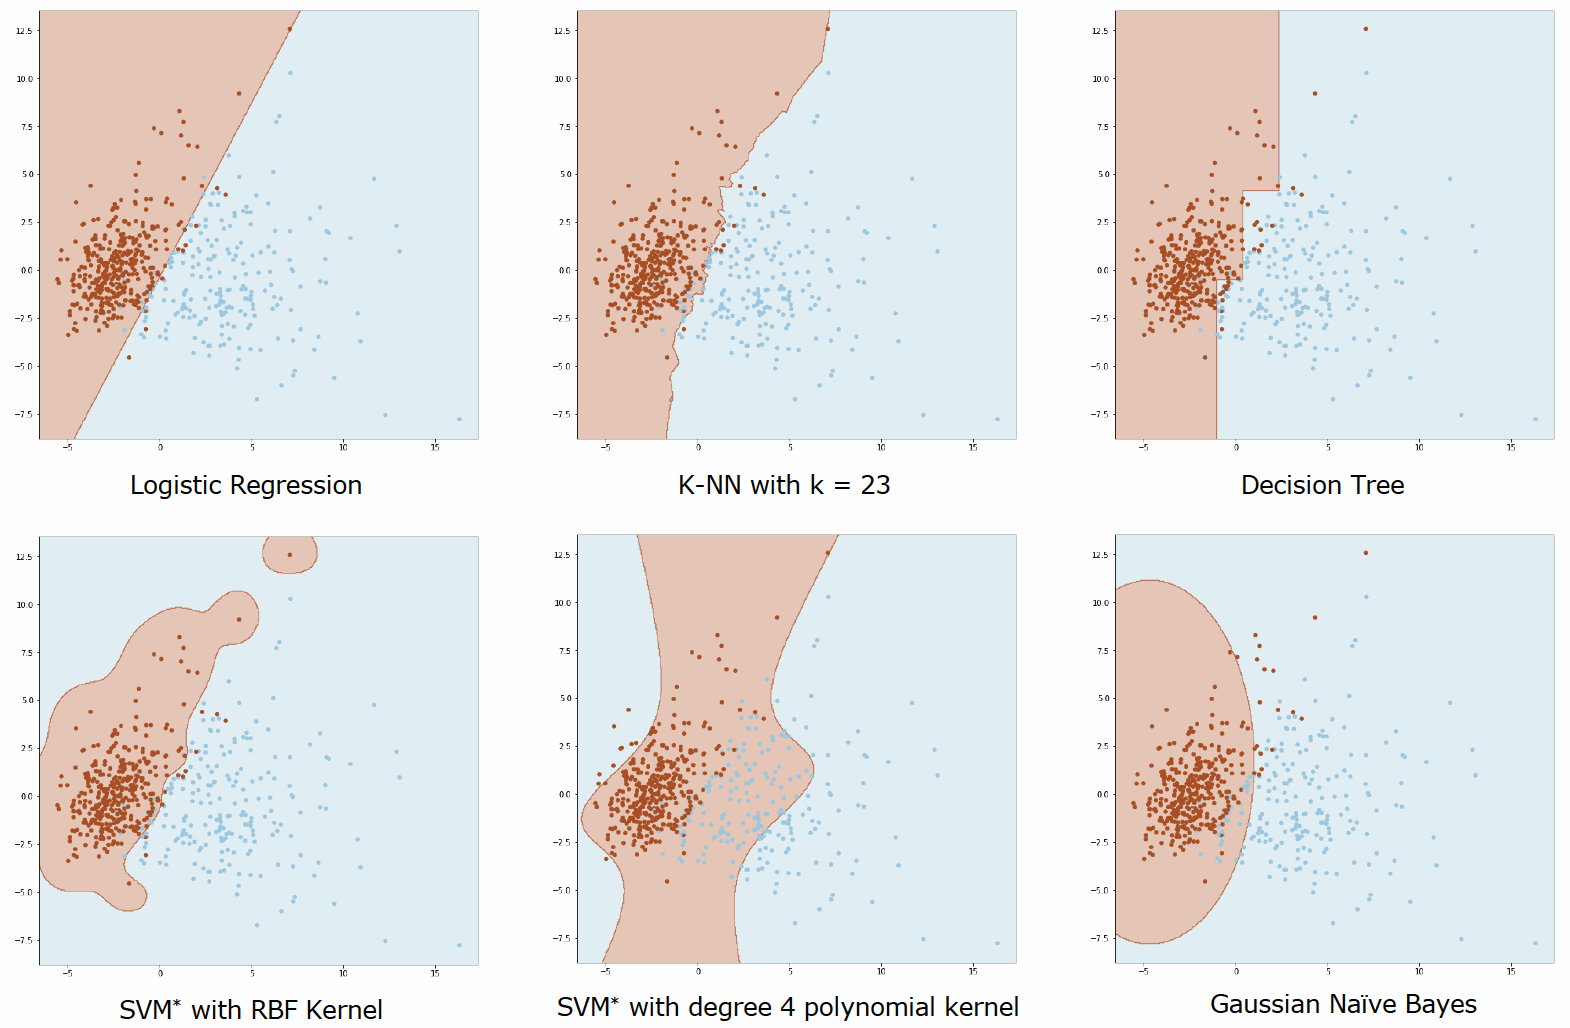
\includegraphics[width=\textwidth]{img/04_supervised_ml/example_class_algos.png}
			\caption{Unterschiede zwischen verschiedenen Classification Algorithmen}
			\label{fig:04_superv_ml_example_class_algos}
		\end{figure}
		
		\newpage
		
		\subsection{Hyperparameters}
		
		Hyperparameter stellen die manuelle Konfiguration von Machine Learning Modellen dar.
		Beispiele von solchen Hyperparametern:
		
		\begin{itemize}
			\item In k-NN ist die Anzahl Nachbarn $k$ ein Hyperparameter
			\item Grad des Polynoms für Regressionsmodelle
			\item Regularisierungsparameter
			\item Kernel für Support-Vektor-Maschinen (SVM)
			\item Tiefe des Baumes und Variablen-Selektions-Policy in Decision Tree Modellen
			\item Anzahl Layers, Neuronen, Aktivierungsfunktion in Deep Learning Modellen
			\item Dropout, Batch Normalisierung, Optimizer etc. in Deep Learning Modellen
		\end{itemize}
	\noindent
		Wenn man als ML-Ingenieur die Hyperparameter-Konfiguration erreichen möchte, welche auf unbekannten Daten am besten performt, kann eine simplistische Train-Test Aufteilung nicht genutzt werden.
		
		\subsection{Simplest Machine Learning Workflow}
		
		\begin{figure}[htb!]
			\centering
			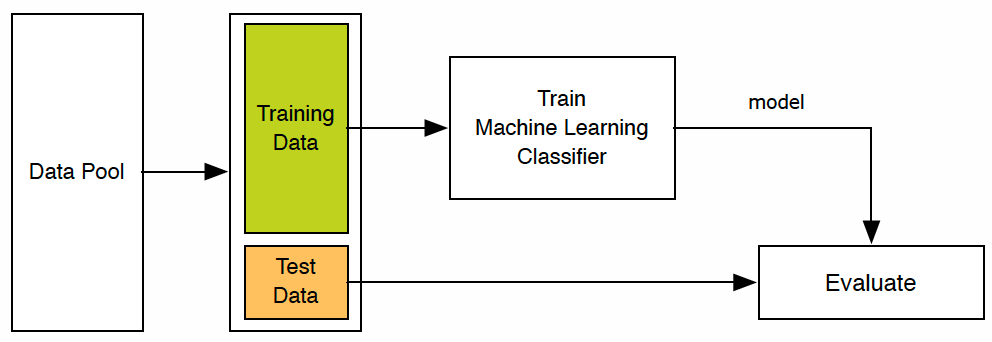
\includegraphics[width=0.6\textwidth]{img/04_supervised_ml/simple_ml.png}
			\caption{Einfachst möglicher ML Workflow}
			\label{fig:04_superv_ml_simple_ml}
		\end{figure}
		
		\begin{itemize}
			\item Daten aufteilen in Trainings- und Test-Set
			\item Trainiere einen Klassifikator auf dem Trainings-Set
			\item Evaluation gibt Rückmeldung über Performance auf einem unbekannten Test-Set
			\item Dies funktioniert nur mit sehr viel Daten und wenn die Hyperparameter fixiert sind
		\end{itemize}
	
		\subsection{Train / Test Splits}
		
		\begin{itemize}
			\item Daten durchmischen (ausser man arbeitet mit Zeitreihen)
			\item Teile die Daten auf in Training- und Test-Set
			\item Empfohlene Aufteilung: 70\% Training / 30\% Test
			\item Training- und Test-Set müsen "disjoint" sein (keine gemeinsamen Elemente haben)
			\item Baue dein Model auf Basis des Training-Set
			\item Evaluiere dein Model auf dem Test-Set
			\item Wenn das Test-Set nicht mehrmals genutzt wurde, gibt es eine Schätzung, wie gut das Modell auf unbekannten Daten performt
		\end{itemize}
	
		\subsection{How to get Fired as a Data Scientist}
		
		\begin{itemize}
			\item Anzahl Nachbarn $k$ ist ein Hyperparameter
			\item Wir optimieren $k$ indem wir testen: $k$ = 1, ... , 10
			\item Für jedes $k$ wird...
			\begin{itemize}
				\item das Modell auf dem Training-Set trainiert
				\item die Performance auf dem Test-Set gemessen
			\end{itemize}
			\item Hyperparameter $k$ = 6 gewinnt, weshalb wir eine Accuracy von 0.99 auf unbekannten Daten erwarten
				$\rightarrow$ \textbf{Diese Schlussfolgerung ist gottverdammt noch mal falsch!}
				\begin{itemize}
					\item Der Hyperparameter ist gewählt basierend auf der Test-Set-Evaluation, demnach basiert dieser logischerweise auf dem Test-Set
					\item Das Test-Set Resultat kann nicht mehr als unverfälschte Schätzung angesehen werden
				\end{itemize}
		\end{itemize}
	
		\subsection{More Complex Evaluation Workflows}
		
		\begin{itemize}
			\item Empfohlene Aufteilung: 60\% Training / 20\% Validation / 20\% Test
			\item Wie evaluiert man einen ML Klassifizierer korrekt:
				\begin{enumerate}
					\item Loop über alle Hyperparameter-Kombinationen, die man ausprobieren möchte
					\item Trainiere das Modell mit ausgewählten Hyperparameter-Einstellungen auf dem \underline{Training-Set}
					\item Evaluiere das Modell auf dem \underline{Validation-Set} und messe die Performance
					\item Wähle das Modell mit der besten Performance als Kandidaten
					\item Evaluiere das Modell auf dem \underline{Test-Set} für eine finale Performance-Schätzung
				\end{enumerate}
			\item Ein solcher Workflow benötigt eine grosse Menge an "guten" Daten
		\end{itemize}
	
		\subsection{Confusion Matrix for Binary Classifiers}
		
		Wir stellen uns einen Klassifizierer vor, welcher die Präsenz von Lungenkrebs voraussagen soll:
		
		\begin{table}[htb!]
			\begin{tabular}{l|l|l|}
				\cline{2-3}
				n=165                             & \textbf{Predicted: NO} & \textbf{Predicted: YES} \\ \hline
				\multicolumn{1}{|l|}{\textbf{Actual: NO}}  & 50            & 10             \\ \hline
				\multicolumn{1}{|l|}{\textbf{Actual: YES}} & 5             & 100            \\ \hline
			\end{tabular}
		\end{table}
	\noindent
		Das Test-Set besteht aus 165 Patientenaufzeichnungen ($n$ = 165)
	
		\begin{itemize}
			\item 50x wurde vom Klassifizierer NO vorausgesagt, die wahre Aussage war tatsächlich NO \\
				$\rightarrow$ Der Klassifizierer hatte recht, dies ist ein \textbf{true-negative (TN)}
			\item 10x wurde vom Klassifizierer YES vorausgesagt, die wahre Aussage war aber NO \\
				$\rightarrow$ Der Klassifizierer lag falsch, dies ist ein \textbf{false-positive (FP)}
			\item 5x wurde vom Klassifizierer NO vorausgesagt, die wahre Aussage war aber YES \\
				$\rightarrow$ Der Klassifizierer lag falsch, dies ist ein \textbf{false-negative (FN)}
			\item 100x wurde vom Klassifizierer YES vorausgesagt, die wahre Aussage war tatsächlich YES \\
				$\rightarrow$ Der Klassifizierer hatte recht, dies ist ein \textbf{true-positive (TP)}
		\end{itemize}
	
		\subsection{Accuracy and Error Rate}
		
		\begin{table}[htb!]
			\begin{tabular}{l|l|l|l}
				\cline{2-3}
				n=165                                      & \textbf{Predicted: NO} & \textbf{Predicted: YES} &                                   \\ \hline
				\multicolumn{1}{|l|}{\textbf{Actual: NO}}  & TN = 50                & FP = 10                 & \multicolumn{1}{l|}{\textit{60}}  \\ \hline
				\multicolumn{1}{|l|}{\textbf{Actual: YES}} & FN = 5                 & TP = 100                & \multicolumn{1}{l|}{\textit{105}} \\ \hline
				& \textit{55}            & \textit{110}            &                                   \\ \cline{2-3}
			\end{tabular}
		\end{table}
	\noindent
		Accuracy misst, wie oft der Klassifizierer richtig lag.\\
		(In diesem Fall: Accuracy = 91\%, Error Rate = 9\%)\\
		
		\begin{itemize}
			\item Accuracy = $\frac{TP + TN}{Total}$\\
			
			\item Error Rate = $\frac{FP + FN}{Total} = 1 - Accuracy$
		\end{itemize}
	
		\paragraph{Accuracy for Imbalanced Data}
		
		\begin{itemize}
			\item Man stelle sich mal vor, man möchte eine seltene Krankheit voraussagen
			\item Ein Test-Set mit 5000 NO- und 20 YES-Aufzeichnungen ist nicht ungewöhnlich...
			\item Der Klassifizierer zeigt eine fantastische Accuracy von 99.6\% - stimmt? Wohl kaum lol
			\item $\rightarrow$ Immer auf Klassen-Unausgeglichenheit überprüfen vor Berechnung der Accuracy!
		\end{itemize}
	
		\newpage
		
		\subsection{Multiclass Classification}
		
		\begin{enumerate}
			\item Einige Algorithmen sind inhärent Multiclass, wie Neurale Netzwerke oder Entscheidungsbäume
			\item Für rein binäre Klassifizierer können wir one-vs-rest Techniken anwenden
				\begin{itemize}
					\item Isoliere Diamanten gegen den Rest
					\item Isoliere Herzen gegen den Rest
					\item Zu guter Letzt, wähle die Klasse wessen Klassifizierer den höchsten Confidence-Score ausgibt
				\end{itemize}
			\item Eine dritte Option wäre hierarchische Klassifizierung
				\begin{enumerate}
					\item Der erste Klassifizierer entscheiden zwischen "Schieben" oder "nicht Schieben"
					\item Der zweite Klassifizierer entscheiden zwischen Trumpf oder {Obe-Abe, Une-Ufe}
					\item etc.
				\end{enumerate}
		\end{enumerate}
	
		\begin{figure}[htb!]
			\centering
			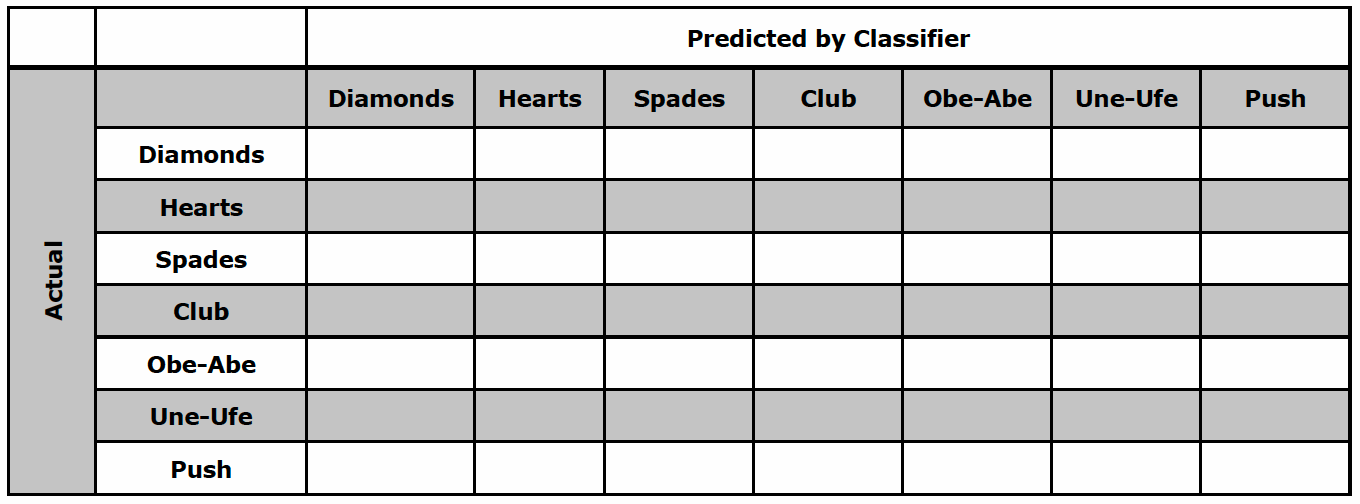
\includegraphics[width=0.6\textwidth]{img/04_supervised_ml/multiclass_confusion_matrix.png}
			\caption{Beispiel einer Multiclass Confusion Matrix am Beispiel vom Jassen}
			\label{fig:04_superv_ml_multiclass_confusion_matrix}
		\end{figure}
	
	\section{Neuronal Networks}
	
		\subsection{AI vs. Machine Learning vs. Deep Learning}
		
		\begin{figure}[htb!]
			\centering
			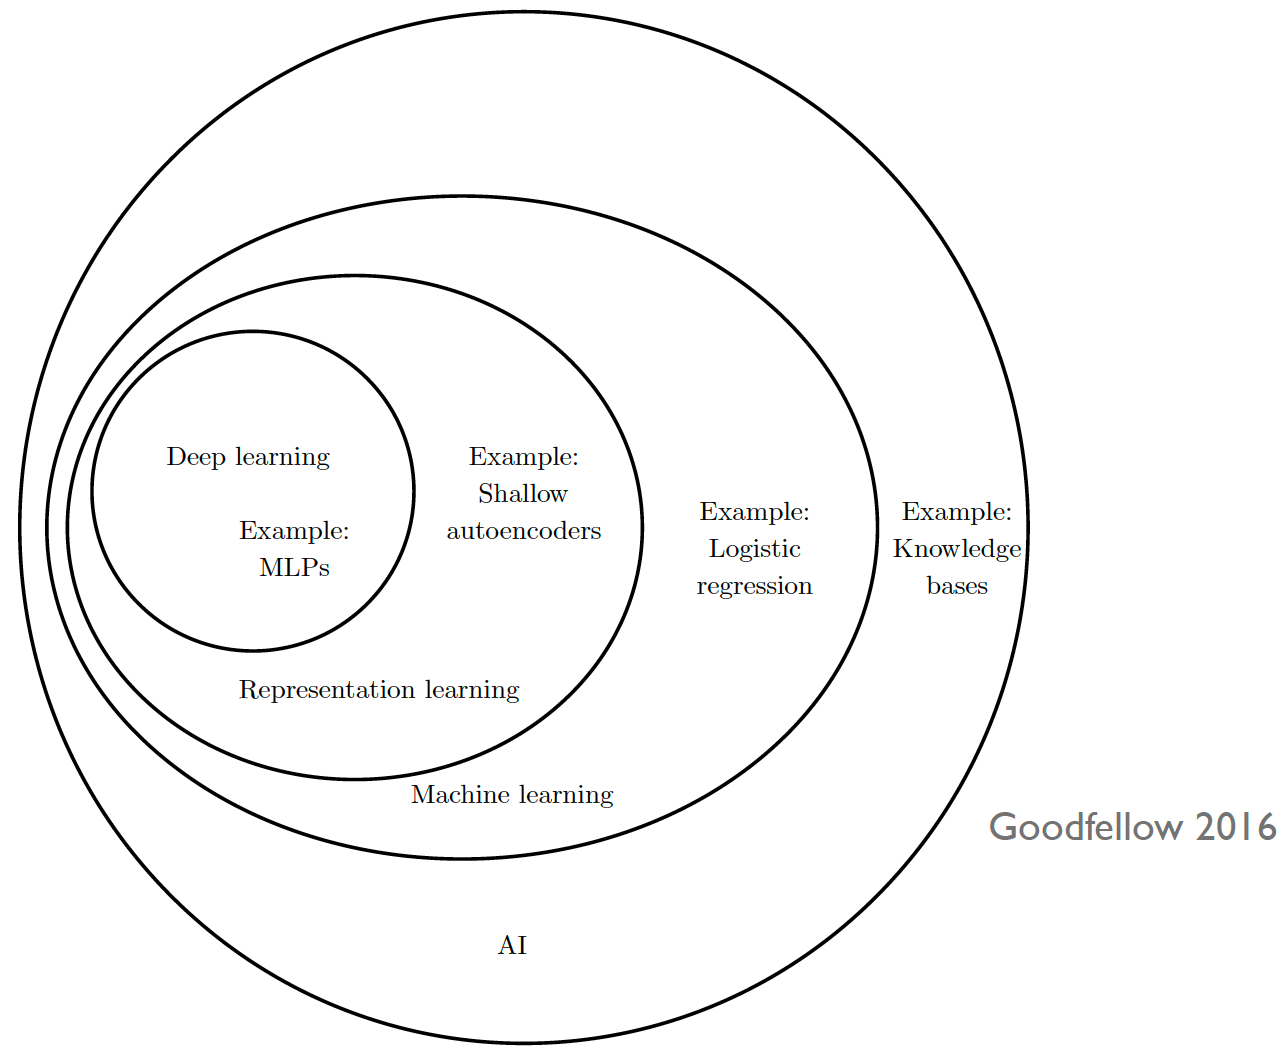
\includegraphics[width=0.7\textwidth]{img/05_neuronal_networks/ai_ml_dl.png}
			\caption{Darstellung der Unterschiede zwischen AI / ML / DL}
			\label{fig:05_neuronet_ai_ml_dl}
		\end{figure}
	
		\newpage
		
		\paragraph{Definition von Machine Learning}
		
		Ein Computerprogramm \textbf{lernt} aus der Experience $E$ mit Rücksicht auf eine Klasse von Tasks $T$ und Performance Measures $P$, wenn es Tasks in $T$ durchführt, gemessen an $P$, seine Experience $E$ verbessert.
		
		\subsection{Task Types}
		
		\begin{itemize}
			\item Regression: $f : \mathbb{R}^{n} \rightarrow \mathbb{R}$ \\
			\item Classification: $f : \mathbb{R}^{n} \rightarrow {1,...,k}$
		\end{itemize}
	
		\subsection{Feed forward Network}
		
		\begin{figure}[htb!]
			\centering
			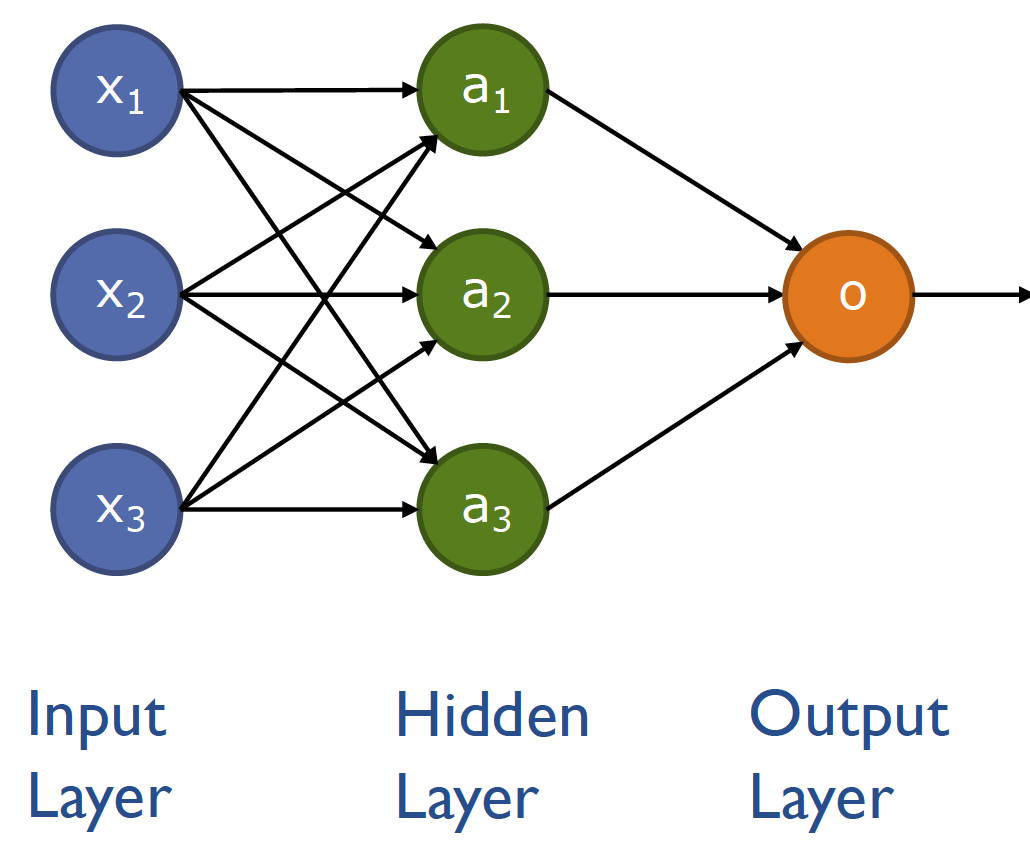
\includegraphics[width=0.5\textwidth]{img/05_neuronal_networks/feed_forward_network.png}
			\caption{Feed Forward Network mit seinen verschiedenen Layers}
			\label{fig:05_neuronet_ff_network}
		\end{figure}
	
		\begin{itemize}
			\item Jeder Knoten $n_{i}$ im Netzwerk hat...
				\begin{itemize}
					\item Inputs $\overline{x} = (x_{1}, ...)$
					\item Interne Parameter $\Theta$
					\item Eine Funktion $y = f_{n_{i}}(\overline{x})$, welche den Output berechnet \\
					(Die Funktion wiederum ist abhängig von den Parametern $\Theta$)
				\end{itemize}
		\end{itemize}
	
		\begin{figure}[htb!]
			\centering
			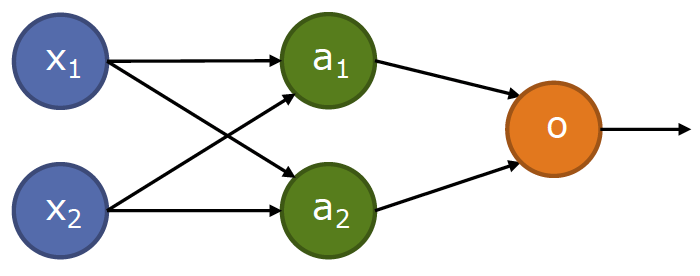
\includegraphics[width=0.3\textwidth]{img/05_neuronal_networks/ffn_rec_calc.png}
			\caption{Feed Forward Network mit kleiner Anzahl Knoten}
			\label{fig:05_neuronet_ffn_rec_calc}
		\end{figure}
	
		Recursive Calculation für ein Feed Forward Network:
		
		$$y = f_{0}(a_{1}, a_{2}) = f_{0}(f_{a_{1}}(x_{1}, x_{2}), f_{a_{2}}(x_{1}, x_{2}))$$
		
		Tiefere neurale Netzwerke haben lediglich mehr Hidden Layers (we need to go deeper $\rightarrow$ $a_{n1}, a_{n_2}, ...$)
		
		\begin{figure}[htb!]
			\centering
			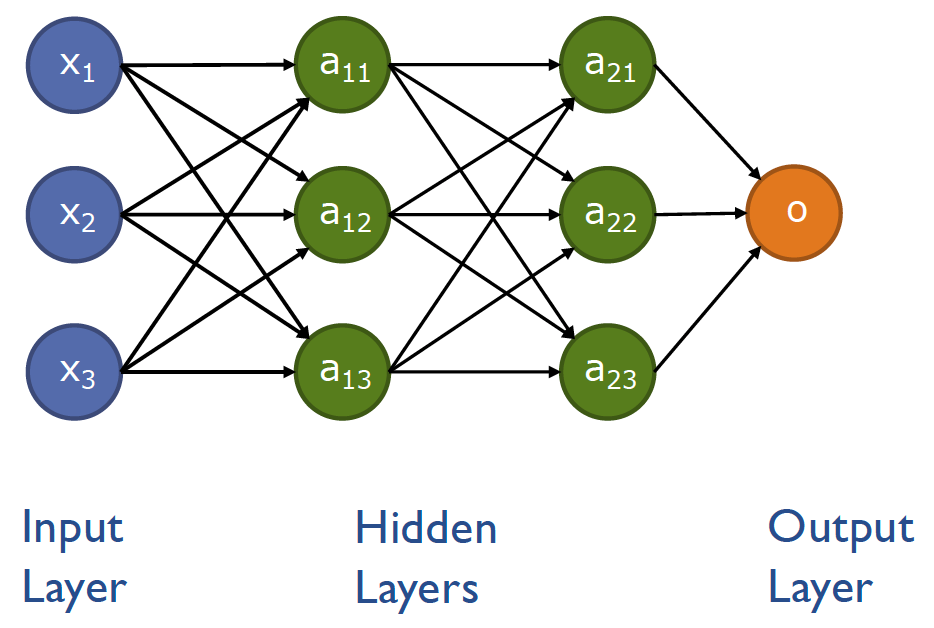
\includegraphics[width=0.3\textwidth]{img/05_neuronal_networks/dnn.png}
		\end{figure}
		
		\newpage
		
		\subsection{Linear Model}
		
		\begin{figure}[htb!]
			\centering
			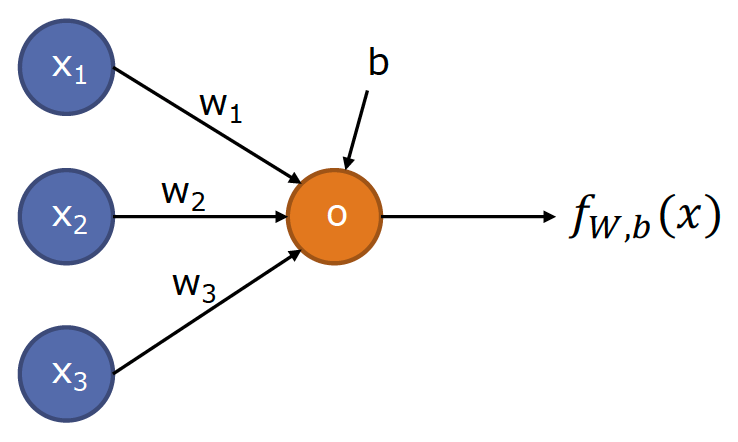
\includegraphics[width=0.4\textwidth]{img/05_neuronal_networks/linear_model.png}
			\caption{Linear Modell eines linearen Neuralen Netzwerks}
			\label{fig:05_neuronet_linear_model}
		\end{figure}
	
		$$f_{W,b}(x) = act(W^{T}x + b)$$
		
		\subsection{Neural network basics in Keras}
		
		Nein, hier sind keine Code-Beispiele aus dem Jupyter-Notebook zu finden.
		Installiert es selber und schaut euch das Beispiel aus dem Unterricht an.
		\begin{itemize}
			\item Lernen wird in \textit{Batches} vollzogen
			\item Eine \textit{Epoche} ist \underline{ein} Traning über das gesamte (Training-)Daten-Set, die Anzahl Epochen hängt vom Task, der Netzwerkkapazität und den Daten ab.
			\item Keras ist ein simples Interface für Beispiele und kleine Tasks, grössere Datensets benötigten meist detailliertere Kontrolle
			\item Keras ist das Standard High-Level Interface von Tensorflow
		\end{itemize}
	
		\subsection{Activation Function}
		
		\begin{itemize}
			\item Sigmoid ist eine gute Wahl für binäre Klassifizierung
			\item Dazwischenliegende Knoten können andere Aktivierungsfunktionen benutzen
			\item Aktivierungsfunktionen sollten non-linear sein
			\item Heutzutage (oder heute?) wird vor allem \textit{relu} als Aktivierungsfunktion für Hidden Layers genutzt
		\end{itemize}
	
		\begin{figure}[htb!]
			\centering
			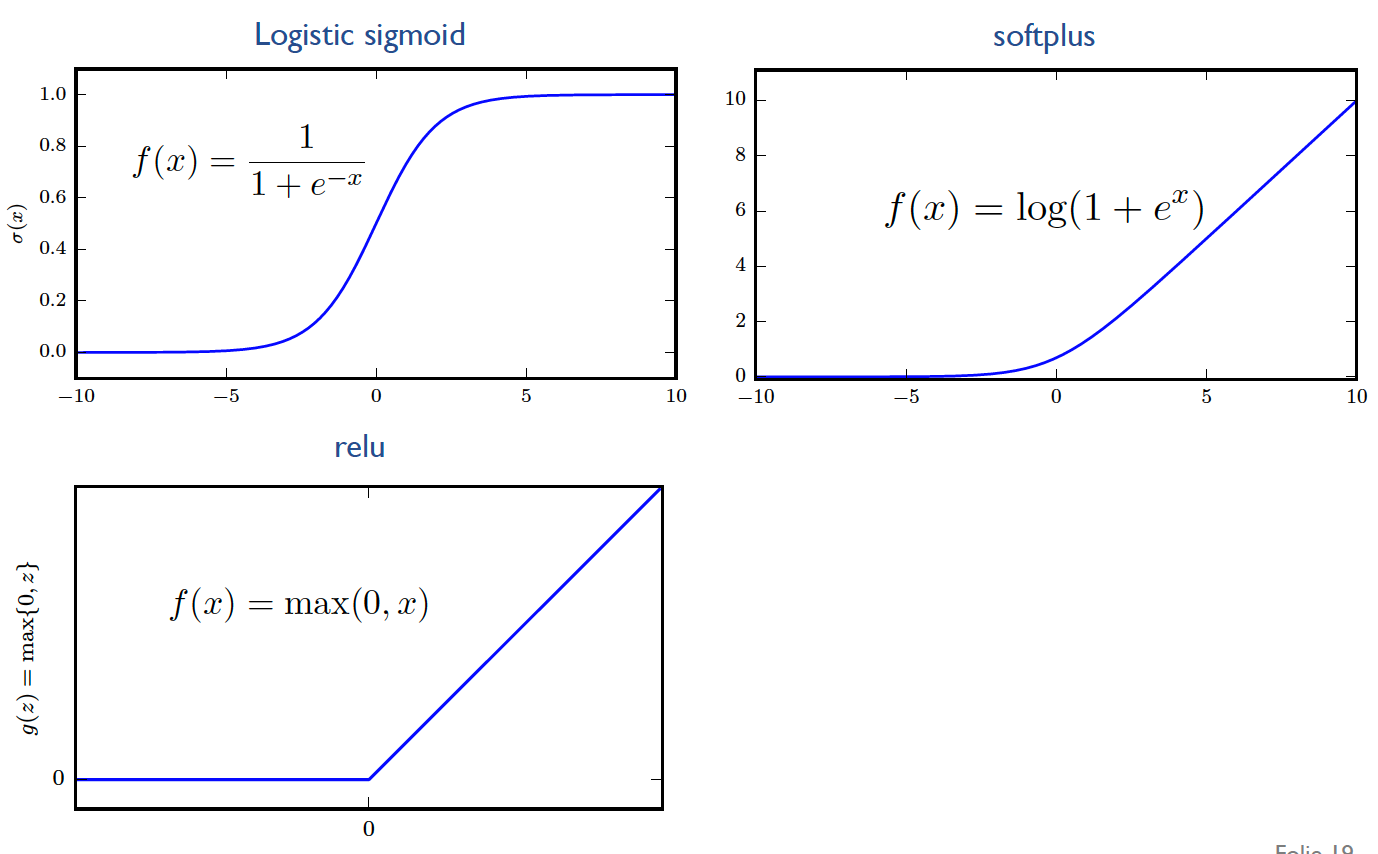
\includegraphics[width=0.8\textwidth]{img/05_neuronal_networks/activation_functions.png}
			\caption{Verschiedene Aktivierungsfunktionen und deren Kurven}
			\label{fig:05_neuronet_activation_functions}
		\end{figure}
		
		\newpage
		
		\subsection{Loss Function}
		
		Loss (oder Kosten-)Funktion ist jene Funktion, welche von den Learning Tasks minimiert werden soll.
		
		\subsection{Likelihood}
		
		\begin{figure*}[htb!]
			\centering
			\begin{subfigure}[b]{0.475\textwidth}
				\centering
				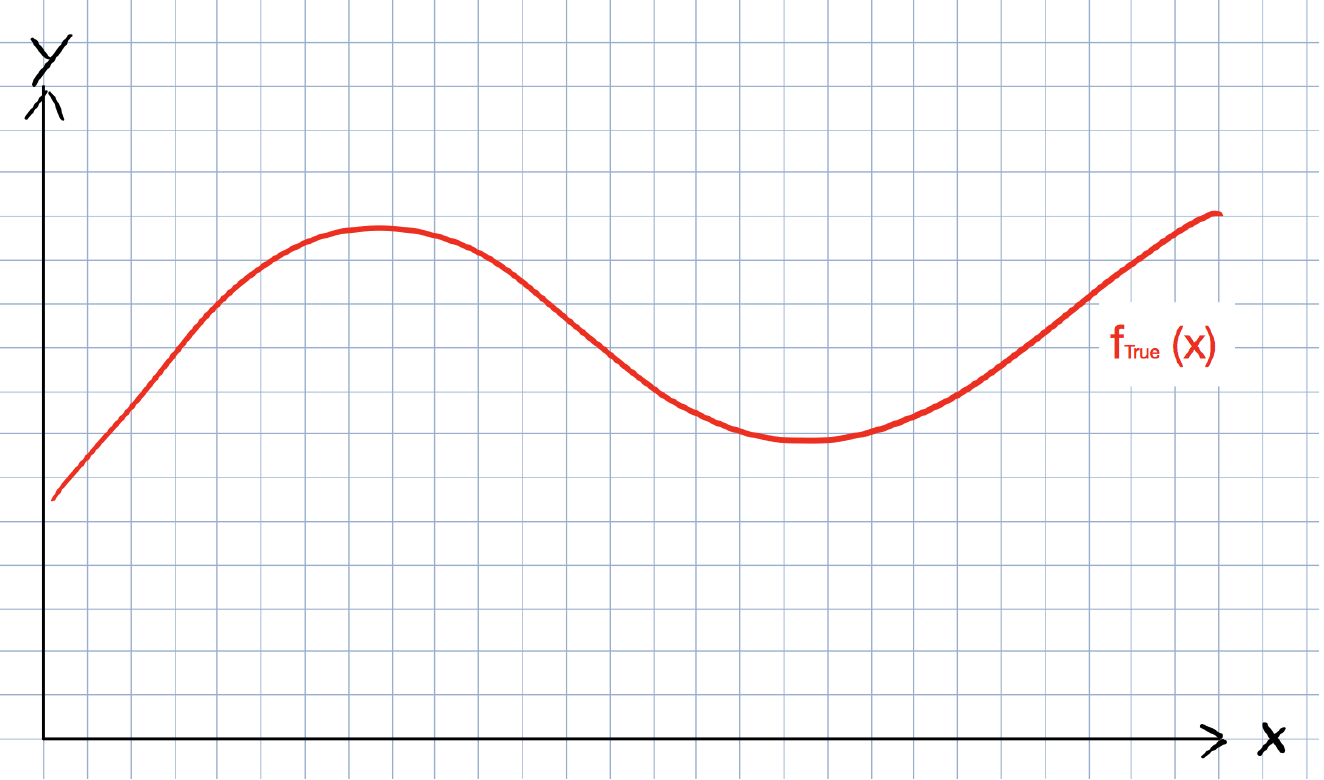
\includegraphics[width=\textwidth]{img/05_neuronal_networks/likelihood_01.png}
			\end{subfigure}
			\hfill
			\begin{subfigure}[b]{0.475\textwidth}
				\centering
				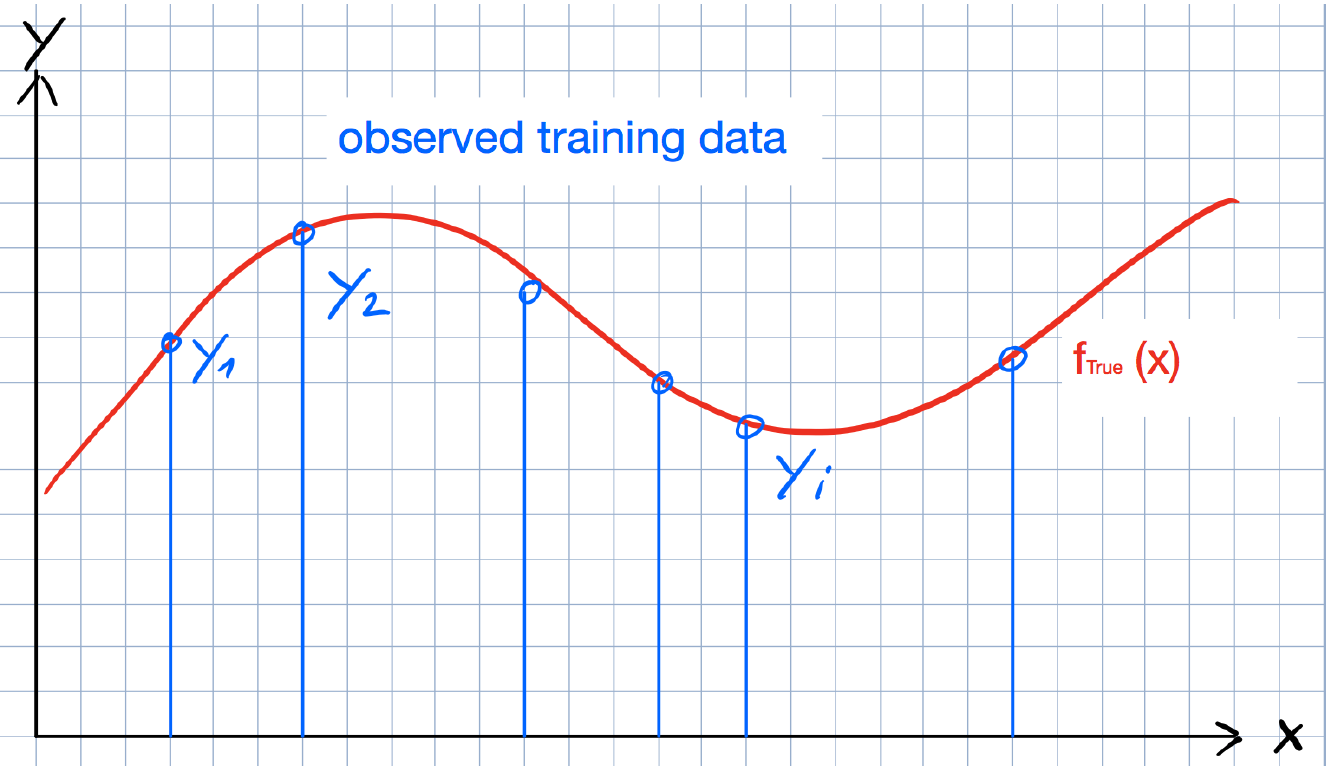
\includegraphics[width=\textwidth]{img/05_neuronal_networks/likelihood_02.png}
			\end{subfigure}
			\vskip \baselineskip
			\begin{subfigure}[b]{0.475\textwidth}
				\centering
				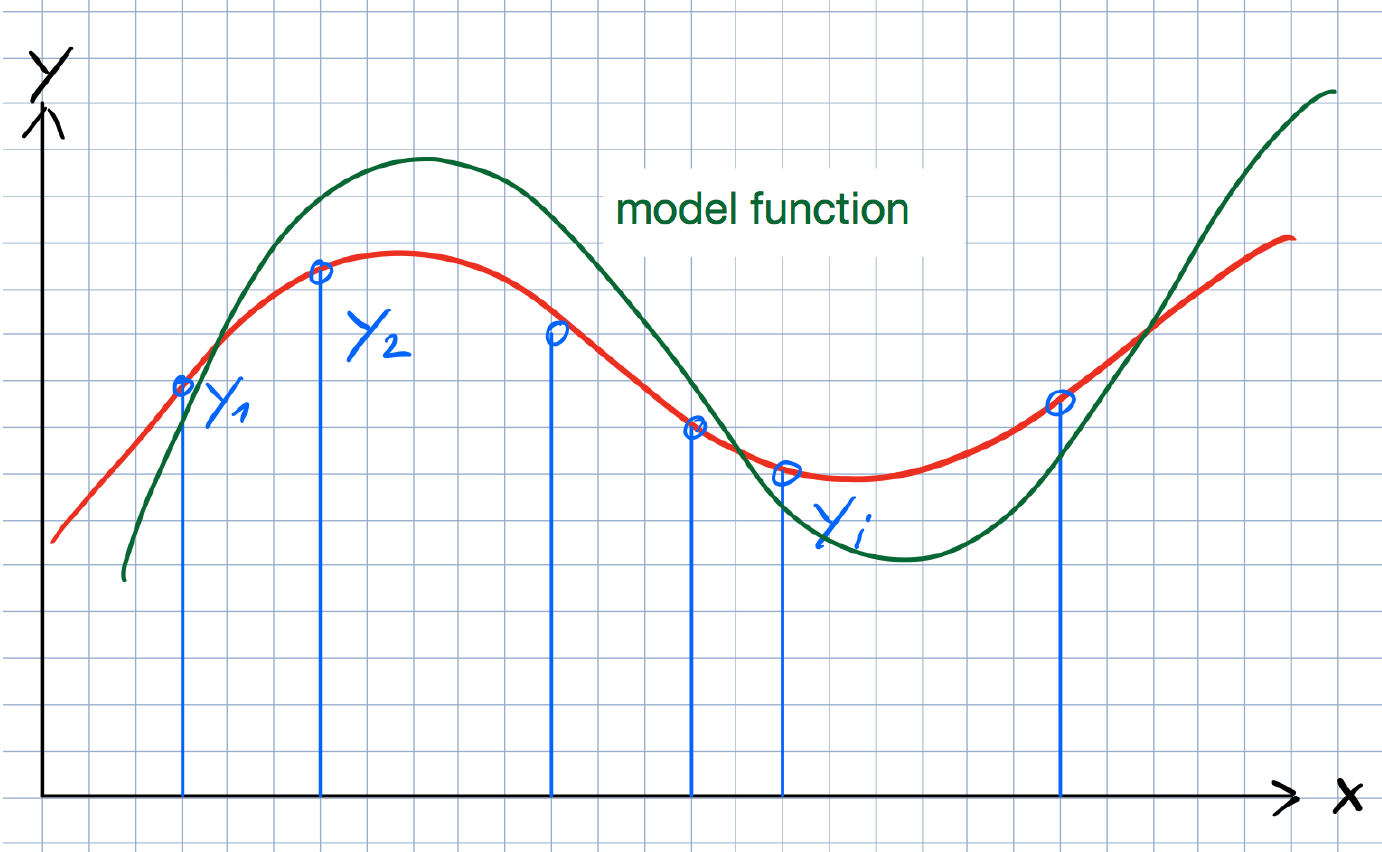
\includegraphics[width=\textwidth]{img/05_neuronal_networks/likelihood_03.png}
			\end{subfigure}
			\quad
			\begin{subfigure}[b]{0.475\textwidth}
				\centering
				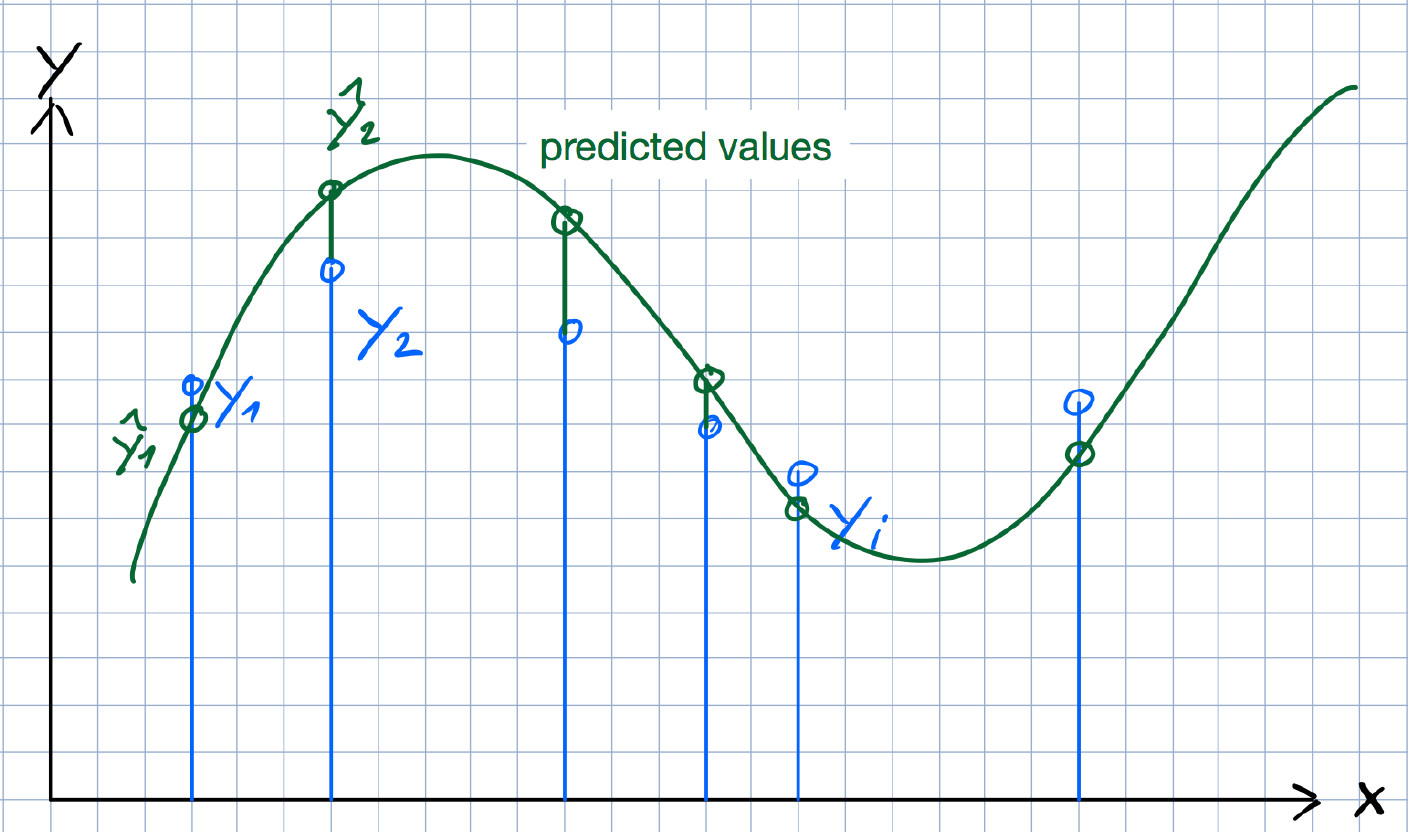
\includegraphics[width=\textwidth]{img/05_neuronal_networks/likelihood_04.png}
			\end{subfigure}
		\end{figure*}
	\noindent
		Was ist die Wahrscheinlichkeit (likelihood), dass die Daten (blaue Kurve) vom Modell (grüne Kurve) produziert wurden?
		Wähle ein Modell, welches diese Likelihood maximiert.
		
		\paragraph{Example: Likelihood}
		
		\begin{itemize}
			\item Werfen einer Münze (Heads, Tails): H = 1, T = 0
			\item $p$: Wahrscheinlichkeit für Head (Modell), die Wahrscheinlichkeit für Tails ist also $(1-p)$ (Bernoulli-Verteilung)
			\item Was ist die Likelihood für ein spezifisches $p$, nach einigen Beobachtungen?
			\item Welches ist das beste Modell $p$ welches zu einer maximalen Likelihood korrespondiert?
			\item Beobachtete Daten:
				\begin{enumerate}
					\item HHH
					\item HHHHHHHHHHHHHHHHHHHHHHHHHH
					\item HHT
				\end{enumerate}
		\end{itemize}
	
		\paragraph{Likelihood}
		
		\begin{itemize}
			\item Maximiere die Likelihood, dass die Daten vom Modell produziert wurden (mit Parameter $\Theta$)
			\item $y_{i}$: Trainingslabel für Punkt $x_{i}$
			\item $\hat{y_{i}}$: Vorausgesagtes Label für Punkt $x_{i}$ (mit Modell $\Theta$)
		\end{itemize}
	
		$$\underset{\Theta}{max}L( y, \hat{y} ) = \prod_{i=0}^{n} L(y_{i}, \hat{y_{i}})$$

		$$ -\log \prod_{i=0}^{n} L(y_{i}, \hat{y_{i}}) = \sum_{i=0}^{n} -\log L(y_{i}, \hat{y_{i}}) $$
		
		\newpage
		
		\subsection{Optimal loss function}
		
		Für kategorische Probleme (Entscheidungen zwischen 0 und 1), ist die optimale Loss Function die Cross Entropy
		
		$$  H_{i} = - ( y_{i} \log( \hat{y_{i}} ) + (1 - y_{i}) \log( 1-\hat{y_{i}} ) ) $$
		
		$$ H = - \sum_{i=0}^{n} ( y_{i} \log ( \hat{y_{i}} ) + ( 1 - y_{i} ) \log ( 1 - \hat{y_{i}} ) ) $$
		
		\subsection{Multi-class problem}
		
		\begin{itemize}
			\item In Multi-Class Klassifizierung wollen wir in eine von $k$ verschiedenen Klassen entscheiden
			\item Für Training und Evaluation: Wir nutzen nicht die Labels direkt, stattdessen nutzen wir One-Hot Encoded oder kategorische Vektoren
		\end{itemize}
	
		\begin{table}[htb!]
			\centering
			\begin{tabular}{|l|l|}
				\hline
				\textbf{Klasse} & \textbf{Vektor} \\ \hline \hline
				0               & (1, 0, 0, 0)    \\ \hline
				1               & (0, 1, 0, 1)    \\ \hline
				2               & (0, 0, 1, 0)    \\ \hline
				3               & (0, 0, 0, 1)    \\ \hline
			\end{tabular}
		\end{table}
	
		\begin{itemize}
			\item Der Output soll für jede Klasse eine Wahrscheinlichkeit annähern
			\item Um dies zu erreichen, nutzen wir die \textit{Softmax} Funktion als Aktivierungsfunktion für den letzten Layer
		\end{itemize}
	
		$$ softmax(z)_{i} = \frac{exp(z_{i})}{\sum_{j} exp(z_{j})} $$
		
		\paragraph{Minimizing a function}
		
		\begin{itemize}
			\item Wie minimieren wir eine Funktion?
			\item Welche Funktionen sind einfacher zu minimieren?
			\item Welche Eigenschaften muss eine Funktion haben, damit wir das Minimum finden können?
			\item Ein Weg: Einen Punkt nehmen, ableiten und determinieren auf welcher Seite die Werte hoch- oder runtergehen, für weitere Punkte der Funktion wiederholen.
		\end{itemize}
	
		\subsection{Gradient descend}
		
		Wie berechnen wir den Gradienten der Loss Funktion? (Kettenregel, Ableitung)
		
		$$ y = f_{0} ( a_1, a_2 ) = f_0 ( f_{a_1} ( x_1, x_2 ), f_{a_2} ( x_1, x_2 ) ) $$
		
		\newpage
		
		\subsection{Back propagation}
		
		Berechnung des Gradienten durch das Netzwerk. Gradient der Loss Funktion, mit Rücksicht auf den Parameter $\Theta$.
		
		\begin{figure}[htb!]
			\centering
			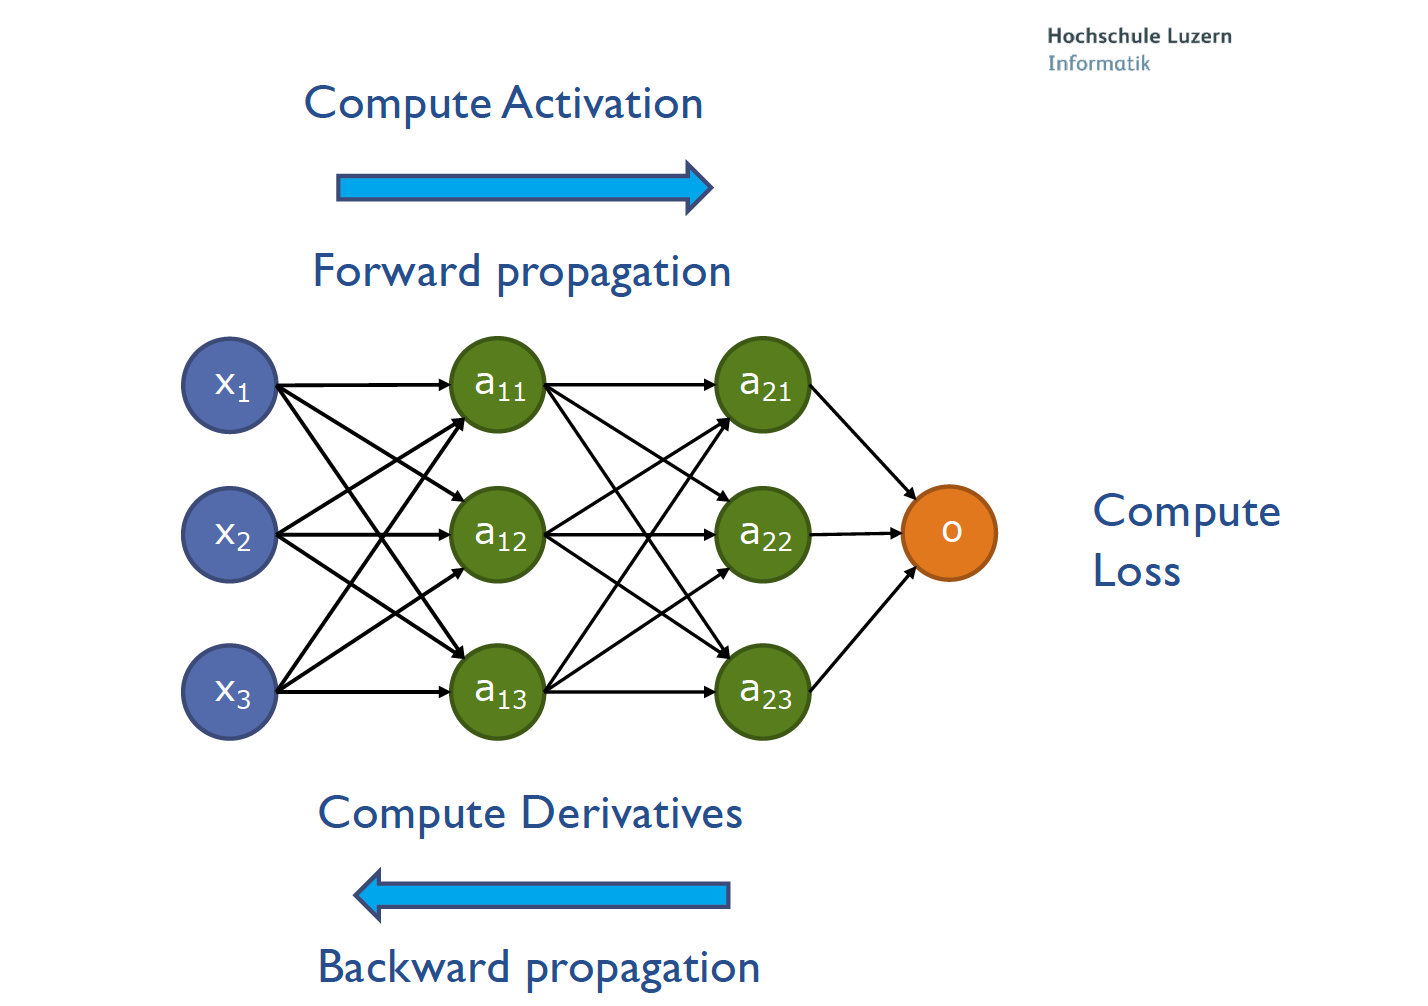
\includegraphics[width=0.5\textwidth]{img/05_neuronal_networks/back_prop.png}
			\caption{Berechnungsvorgang in einem neuralen Netzwerk}
			\label{fig:05_neuronet_back_prop}
		\end{figure}
		
	
	\section{Deep Neuronal Networks}
	
		\subsection{Review Questions}
		
		\begin{itemize}
			\item \textbf{Was ist ein Neurales Netzwerk?} \\
				Ein neurales Netzwerk enthält verschiedene Layers, welche verschiedene Funktionen mit verschiedenen Parametern haben.
				Ein Neuron ist eine lineare Funktion (bspw. \textit{relu} ($w \cdot x + b$ wobei $x$ = Input, Werte des letzten Layers, $w$ = Gewicht der Verbindung, $b$ = Bias (wird vom Netzwerk gelernt)))
			\item \textbf{Wie berechnet ein Neurales Netzwerk ein Resultat?} \\
				Es versucht den Loss zu minimieren (mit einer Loss Funktion)
			\item \textbf{Was ist eine Loss Funktion?} \\
				Phaha kei Blame.
				%TODO
			\item \textbf{Wie wird ein Neurales Netzwerk trainiert?} \\
				Backpropagation wird genutzt um die Gewichte zu verbessern (funktioniert dank der Kettenregel) und Gradient Descend wird verwendet. Erst wird versucht, die Accuracy zu verbessern, danach die Loss Funktion.
			\item \textbf{Wie weisst du, dass das Training erfolgreich war?} \\
				Durch die Resultate der Evaluation mit dem Test-Set.
		\end{itemize}
	
		\subsection{Deeper neuronal Networks}
		
		\begin{itemize}
			\item Deeper $\rightarrow$ Representation Learning
			\item NN: $Features \rightarrow Outputs$
			\item DNN: $Raw Input \rightarrow Features \rightarrow Output$
		\end{itemize}
		
		\paragraph{Capacity}
		
		Wie gross/tief/weit sollte ein Netzwerk sein?
		
		\begin{figure*}[htb!]
			\centering
			\begin{subfigure}[b]{0.475\textwidth}
				\centering
				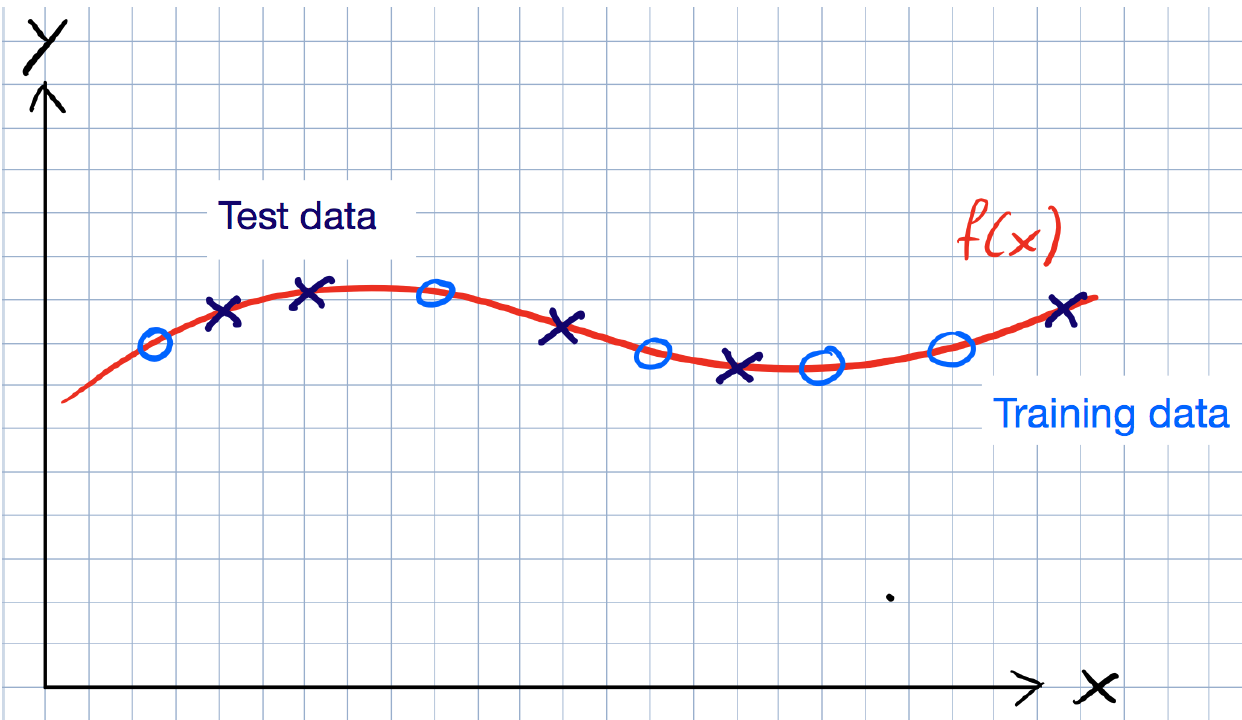
\includegraphics[width=0.6\textwidth]{img/06_deep_nn/capacity_01.png}
			\end{subfigure}
			\hfill
			\begin{subfigure}[b]{0.475\textwidth}
				\centering
				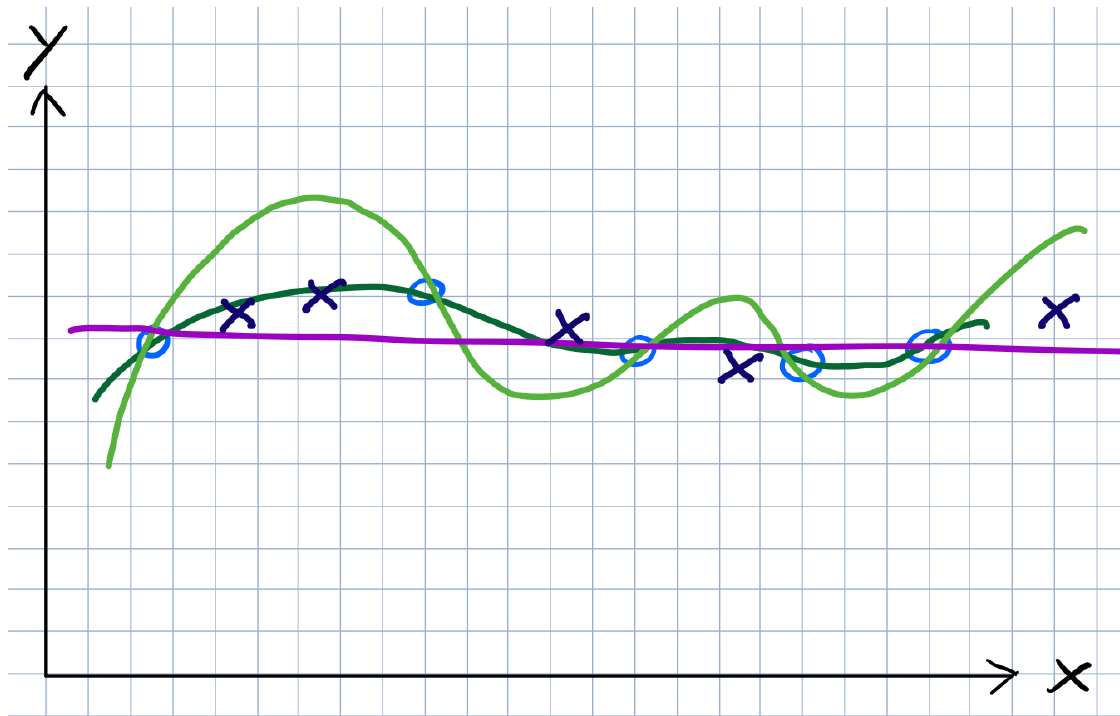
\includegraphics[width=0.6\textwidth]{img/06_deep_nn/capacity_02.png}
			\end{subfigure}
		\end{figure*}
		
		\newpage
		
		\subsection{Errors}
		
		\begin{itemize}
			\item \textbf{Training Error}: Fehler auf dem Training-Set
			\item \textbf{Generalization Error}: Lücke zwischen Fehler auf Training- und Test-Set
			\item \textbf{Underfitting}: Grosser Bias, nicht genug Kapazität, grosser Fehler auf Training- (und Test-)Set
			\item \textbf{Overfitting}: Grosse Varianz, zu viel Kapazität, kleiner Fehler auf Training-, aber grosser Fehler auf Test-Set $\rightarrow$ Large Generalization Error
		\end{itemize}
	
		\subsection{Optimal Capacity}
		
		\begin{figure}[htb!]
			\centering
			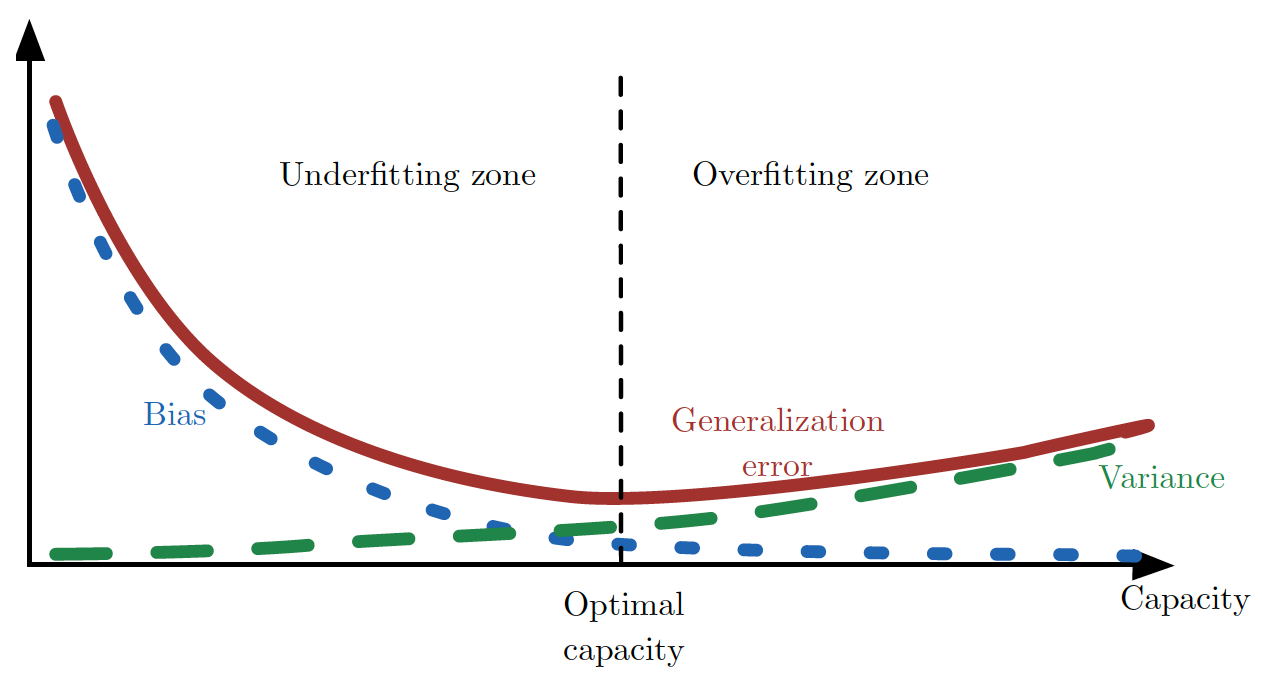
\includegraphics[width=0.6\textwidth]{img/06_deep_nn/optimal_capacity.png}
			\caption{Wahl der optimalen Kapazität, um Fehler auszugleichen}
			\label{fig:06_deep_nn_optimal_capacity}
		\end{figure}
	
		\subsection{Regularization}
	\noindent
		Limitiere die Kapazität des Netzwerks, indem eine Parameter Norm Penalty zum Loss hinzugefügt wird.
		
		\begin{figure}[htb!]
			\centering
			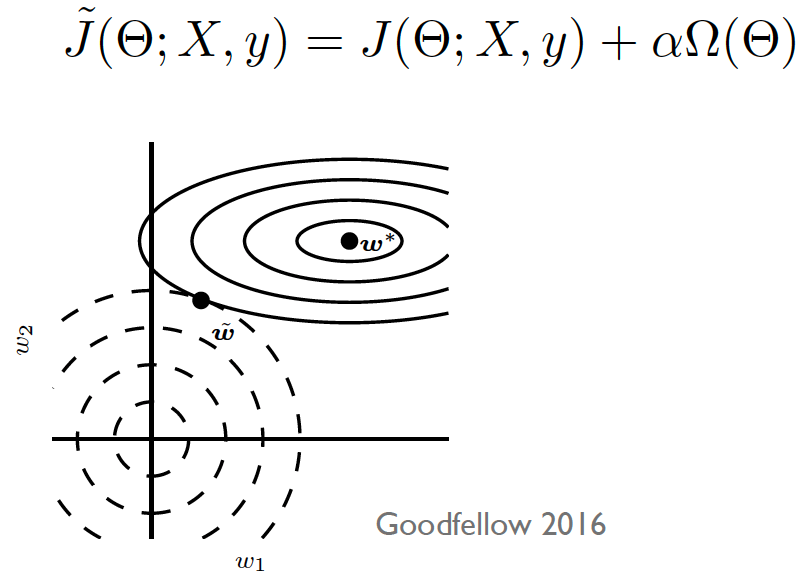
\includegraphics[width=0.4\textwidth]{img/06_deep_nn/regularization.png}
		\end{figure}
	
		\begin{figure*}[htb!]
			\centering
			\begin{subfigure}[b]{0.475\textwidth}
				\centering
				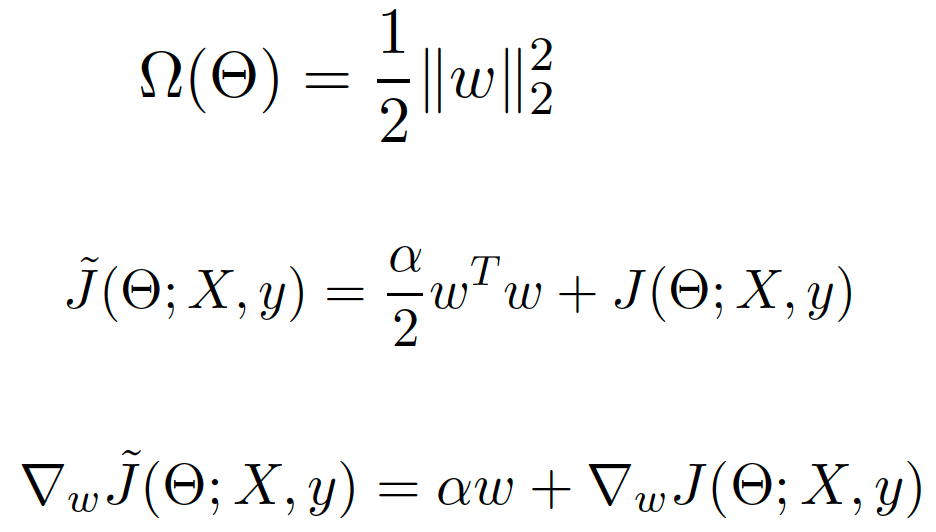
\includegraphics[width=0.8\textwidth]{img/06_deep_nn/l2_regularization.png}
				\caption{$L^2$ Regularisierung}
			\end{subfigure}
			\hfill
			\begin{subfigure}[b]{0.475\textwidth}
				\centering
				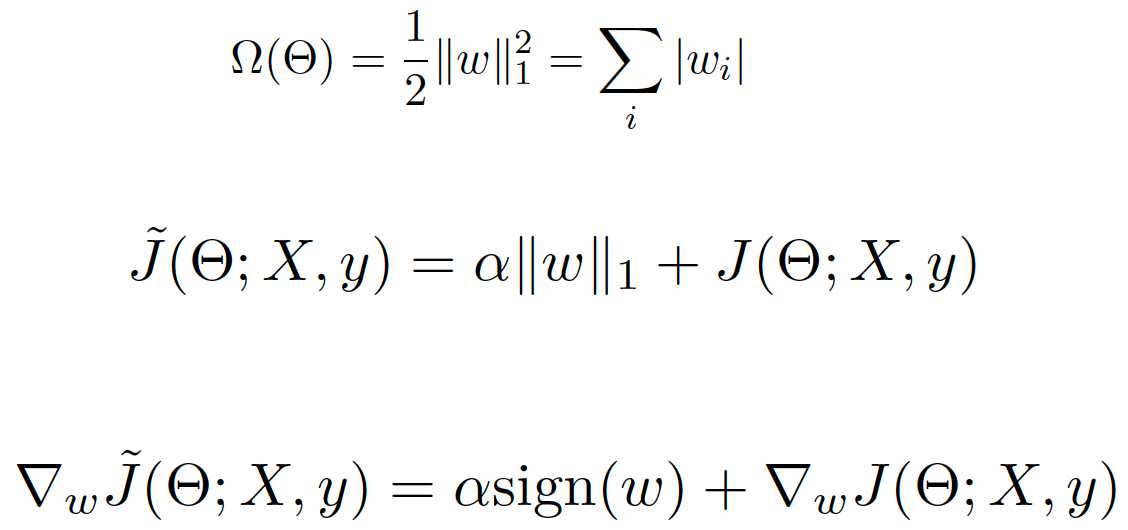
\includegraphics[width=\textwidth]{img/06_deep_nn/l1_regularization.png}
				\caption{$L^1$ Regularisierung}
			\end{subfigure}
		\end{figure*}
	
		\newpage
	
		\paragraph{Other regularization}
		
		\begin{itemize}
			\item Ensemble Methods
				\begin{itemize}
					\item Nutze einige Modelle, welche separat trainiert werden, und stimme dann auf das Resultat ab
				\end{itemize}
			\item Dropout
				\begin{itemize}
					\item Entferne einen zufälligen Knoten, aus einem Hidden Layer, oder einen Eingabewert \\
						(Im Grunde genommen, multipliziere das Resultat dieses Knoten mit 0)
					\item Das Training lernt alle Sub-Netzwerke des originalen Netzwerks
				\end{itemize}
			\item Early Stopping
				\begin{itemize}
					\item Stoppe, wenn der Fehler auf dem Validation-Set wieder zu wachsen beginnt
					\item Im Grunde genommen, lerne die benötigte Anzahl Training-Steps (als Hyperparameter)
				\end{itemize}
		\end{itemize}
	
		\begin{figure*}[htb!]
			\centering
			\begin{subfigure}[b]{0.475\textwidth}
				\centering
				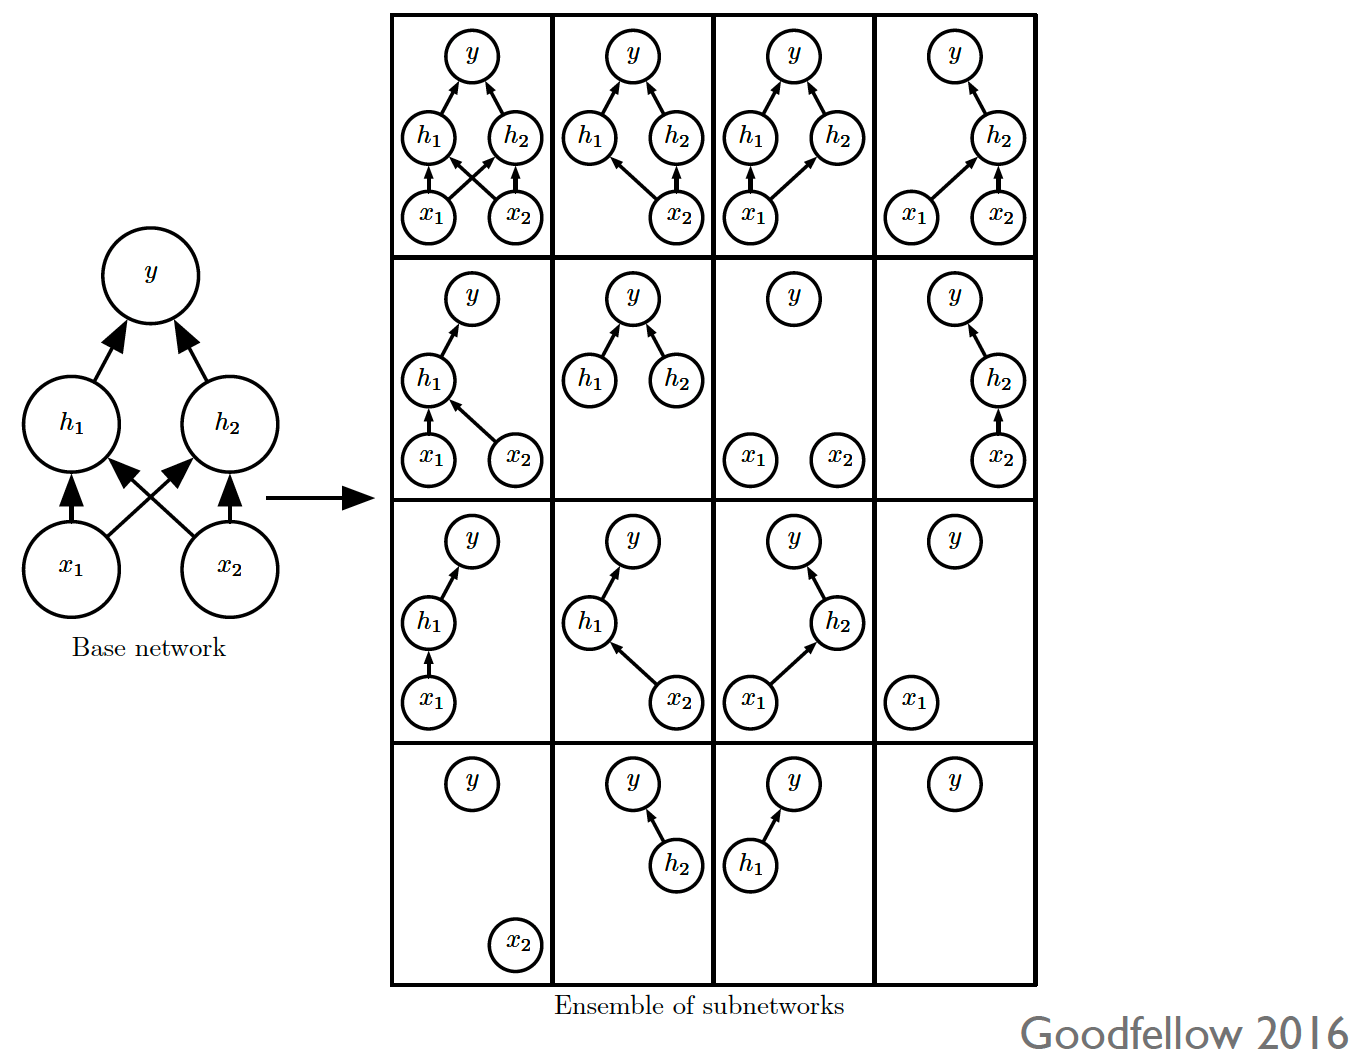
\includegraphics[width=\textwidth]{img/06_deep_nn/dropout.png}
				\caption{Dropout Regularisierung}
			\end{subfigure}
			\hfill
			\begin{subfigure}[b]{0.475\textwidth}
				\centering
				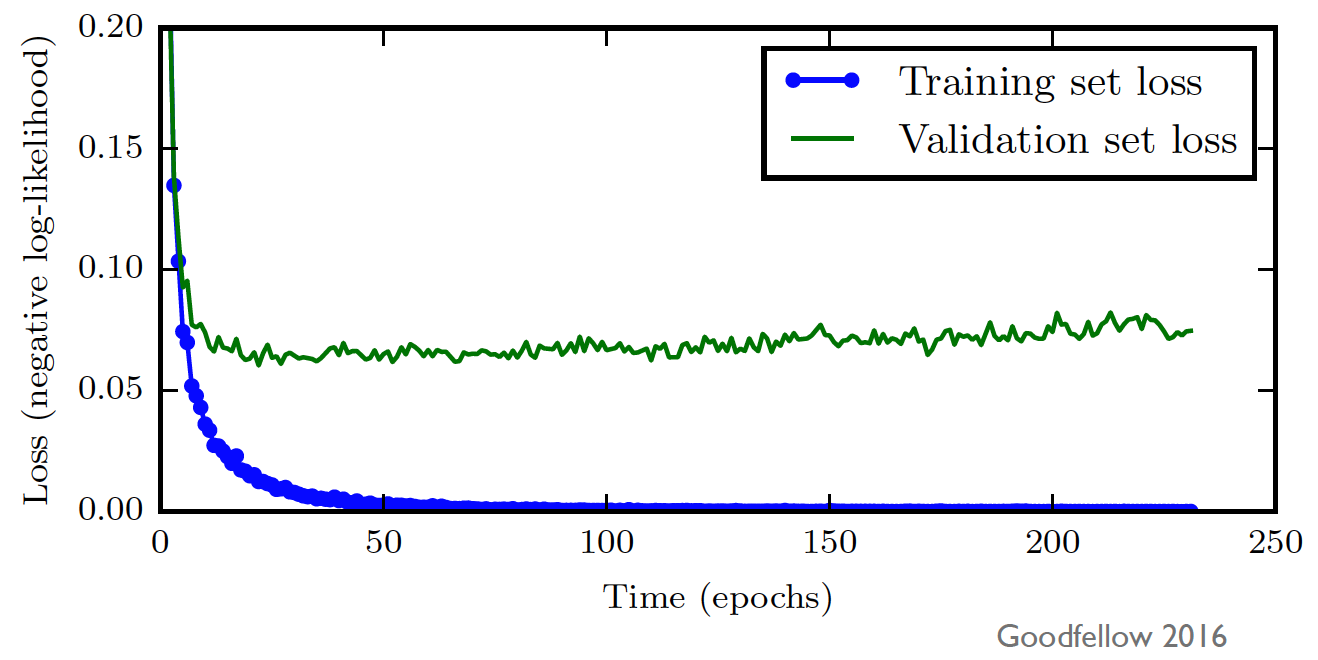
\includegraphics[width=\textwidth]{img/06_deep_nn/early_stopping.png}
				\caption{Early Stopping Regularisierung}
			\end{subfigure}
		\end{figure*}
		
		
	
	
		
		
	
	\section{Convolutional Neuronal Networks}
	
	
	
	\section{Reinforcement Learning}
	
	
	
	
\end{document}
